\documentclass[master]{suribt}
\usepackage{url}
\usepackage{graphicx}
\usepackage{algorithm}
\usepackage{algorithmicx}
\usepackage[noend]{algpseudocode}
\usepackage{amsmath}
\usepackage{amssymb}
\usepackage{amsthm}
\usepackage{latexsym}

\theoremstyle{definition}
\newtheorem{thm}{定理}
\newtheorem{defi}[thm]{定義}
\newtheorem{prop}[thm]{命題}
\newtheorem{cor}[thm]{系}
\newtheorem{asm}[thm]{仮定}

\renewcommand{\algorithmicrequire}{\textbf{Input:}}
\renewcommand{\algorithmicensure}{\textbf{Output:}}
\newcommand{\argmax}{\mathop{\rm argmax}\limits}
\newcommand{\argmin}{\mathop{\rm argmin}\limits}
\newcommand{\tabincell}[2]{\begin{tabular}{@{}#1@{}}#2\end{tabular}}
%\documentclass[oneside]{suribt}% 本文が * ページ以下のときに (掲示に注意)
\title{特許検索における質問意図の曖昧化}
%\titlewidth{}% タイトル幅 (指定するときは単位つきで)
\author{胡瀚林}
\eauthor{HANLIN HU}% Copyright 表示で使われる
\studentid{48-156229}
\supervisor{中川裕志 教授}% 1 つ引数をとる (役職まで含めて書く)
%\supervisor{指導教員名 役職 \and 指導教員名 役職}% 複数教員の場合,\and でつなげる
\handin{2017}{01}% 提出月. 2 つ (年, 月) 引数をとる
%\keywords{キーワード1, キーワード2} % 概要の下に表示される

\begin{document}
\maketitle%%%%%%%%%%%%%%%%%%% タイトル %%%%

\frontmatter% ここから前文
\begin{abstract}%%%%%%%%%%%%% 概要 %%%%%%%%
 企業が特許を取る前に,類似な特許が既に存在するかを確かめるために特許データベースを検索する必要がある.
 しかし,検索の質問から企業秘密が漏洩する可能性がある.
 ウェブテキスト検索の質問からユーザーの検索意図を守る手法が多数存在している.
 その中真の質問と同時にダミー質問を提出する質問曖昧化手法が一番効率的、現実的である.
 本論文では特許検索における既存な質問曖昧化手法\cite{providing2009,embellishing2010,masking2014}を実装し,
 類似度攻撃\cite{simattack2016}で特許データベースにおける既存手法の安全性を評価した.

 また、類似度攻撃\cite{simattack2016}を含め、多くの既存な質問曖昧化に対する攻撃手法は攻撃者が質問者の事前情報を持つと仮定する.
 本論文では事前情報なしの攻撃手法を提案し,その攻撃手法に対応できる既存な質問曖昧化の改良と新たな質問曖昧化手法を提案する.
\end{abstract}

 \tableofcontents%%%%%%%%%%%%% 目次 %%%%%%%%

 \mainmatter% ここから本文 %%% 本文 %%%%%%%%
 \chapter{はじめに}

 テキスト検索をするとき,検索質問をサーバー側に渡さなければならない.
 しかし,検索質問から質問者の情報が漏洩する危険があることがAOL事件\cite{AOL}より証明された.
 特許検索の場合は検索質問が研究開発動向など企業秘密を含んでいるため,一般的なウェブ検索の質問者より質問のプライバシー問題を重視している.
 そのような問題を解く様々な手法が存在している.
 \cite{tor2004}や\cite{private2007}などのIPアドレスの匿名化メカニズムは登録情報が必要な検索サーバーに対応できない.
 また検索質問のみから質問者を一意に特定されてしまう可能性がある.
 プライベート情報検索(Private Information Retrieval)\cite{pir1998}は計算量的安全性を持つが,サーバー側で大量の計算が必要であるため実用するのは難しい.
 曖昧化検索(Obfuscation Search)\cite{obs2012}は真の質問を分析し適切な$K−1$個のダミー質問を生成し真の質問と同時に検索する.
 安全性が弱いが,効率よく質問者の検索意図を守ることができる.
 %またサーバー側の調整の必要がないため検索結果に影響がない.
 

 本論文の構成は次の通りである.
 第二章では特許文章と特許検索の特徴を述べる.
 第三章では既存な質問曖昧化メカニズム\cite{providing2009,embellishing2010,masking2014}を述べる.
 第四章では曖昧化メカニズムがよく用いる意味分析手法を述べる.
 第五章では既存な攻撃手法\cite{simattack2016}を述べ,\cite{simattack2016}の改良と新たな攻撃手法を提案する.
 第六,七章では新たな質問曖昧化手法を提案する.
 最後に, 第八章で評価実験を述べ,第九章で全体をまとめる.


 \chapter{特許}
 特許検索質問のプライバシーを保護する手法を説明する前に特許検索と特許そのものを簡単に紹介する必要がある.
 特許法第1条には,「この法律は、発明の保護及び利用を図ることにより、発明を奨励し、もつて産業の発達に寄与することを目的とする」とある.
 特許制度は,発明者には一定期間,一定の条件のもとに特許権という独占的な権利を与えて発明の保護を図る一方,
 その発明を公開して利用を図ることにより新しい技術を人類共通の財産としていくことを定めて,
 これにより技術の進歩を促進し,産業の発達に寄与しようというものである.\cite{patent}
 特許を取るには以下の条件を満たさなければならない:
 \begin{enumerate}
 \item {\em (新規性:特許法29条第1項)}特許出願前に公然知られた発明,公然実施をせれた発明,頒布された刊行物に記載された発明又は電気通信回線を通じて公衆に利用可能となった発明について特許を受けることができない.
 \item {\em (進歩性:特許法29条第2項)}特許出願前にその発明の属する技術の分野における通常の知識を有する者が前項各号に掲げる発明に基いて容易に発明をすることができたときは、その発明については、同項の規定にかかわらず、特許を受けることができない。
 \end{enumerate}
 %単一性:発明の単一性の要件を満たさない二以上の発明は一つの願書で出願することができない.

 すなわち,特許を出願する前に既存な特許を検索し,自分の発明について新規性と進歩性の有無を判断する必要がある.また,特許を受けようとする新規性と進歩性がある発明を特定られる特許請求の範囲を記載する必要がある.
 \begin{figure}
  \hspace*{-2cm}
  \begin{tabular}{cc}
  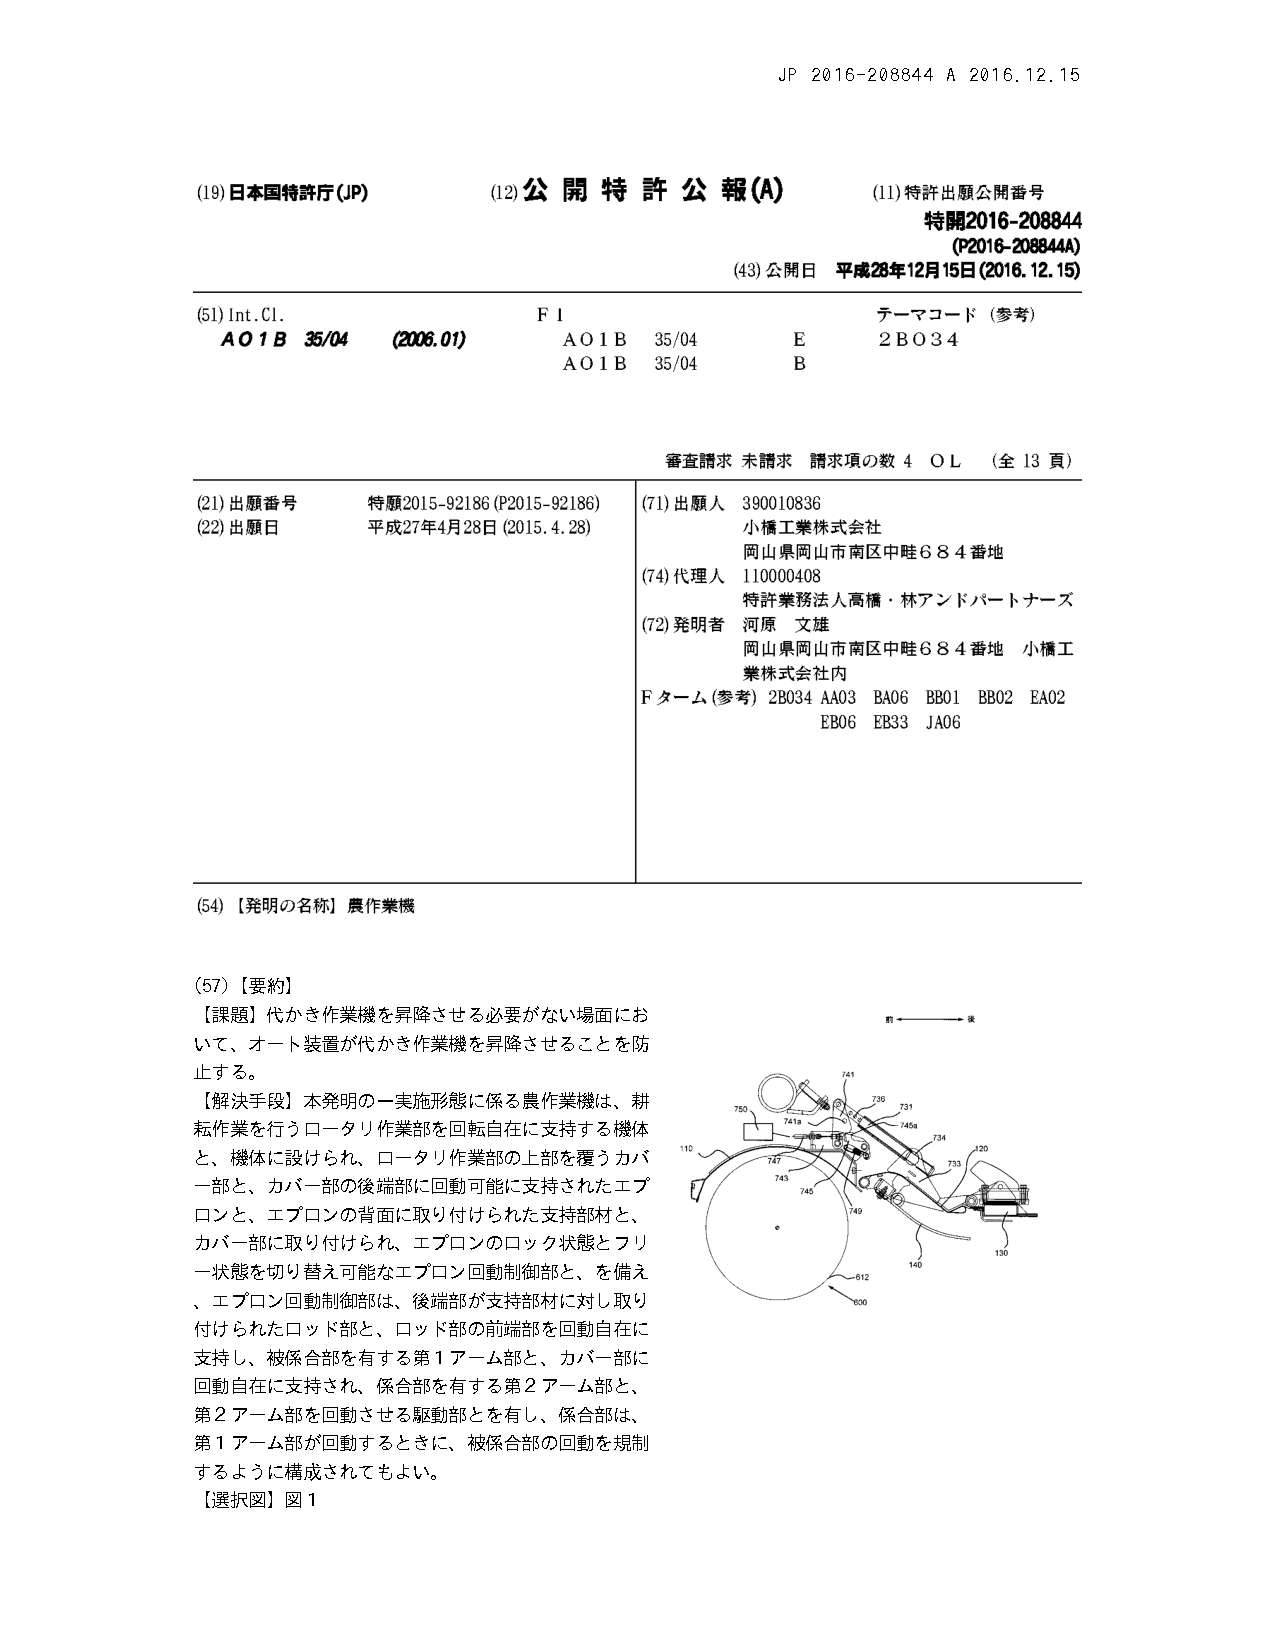
\includegraphics[width=0.55\textwidth,natwidth=500,natheight=1100]{ex1-1.pdf}
  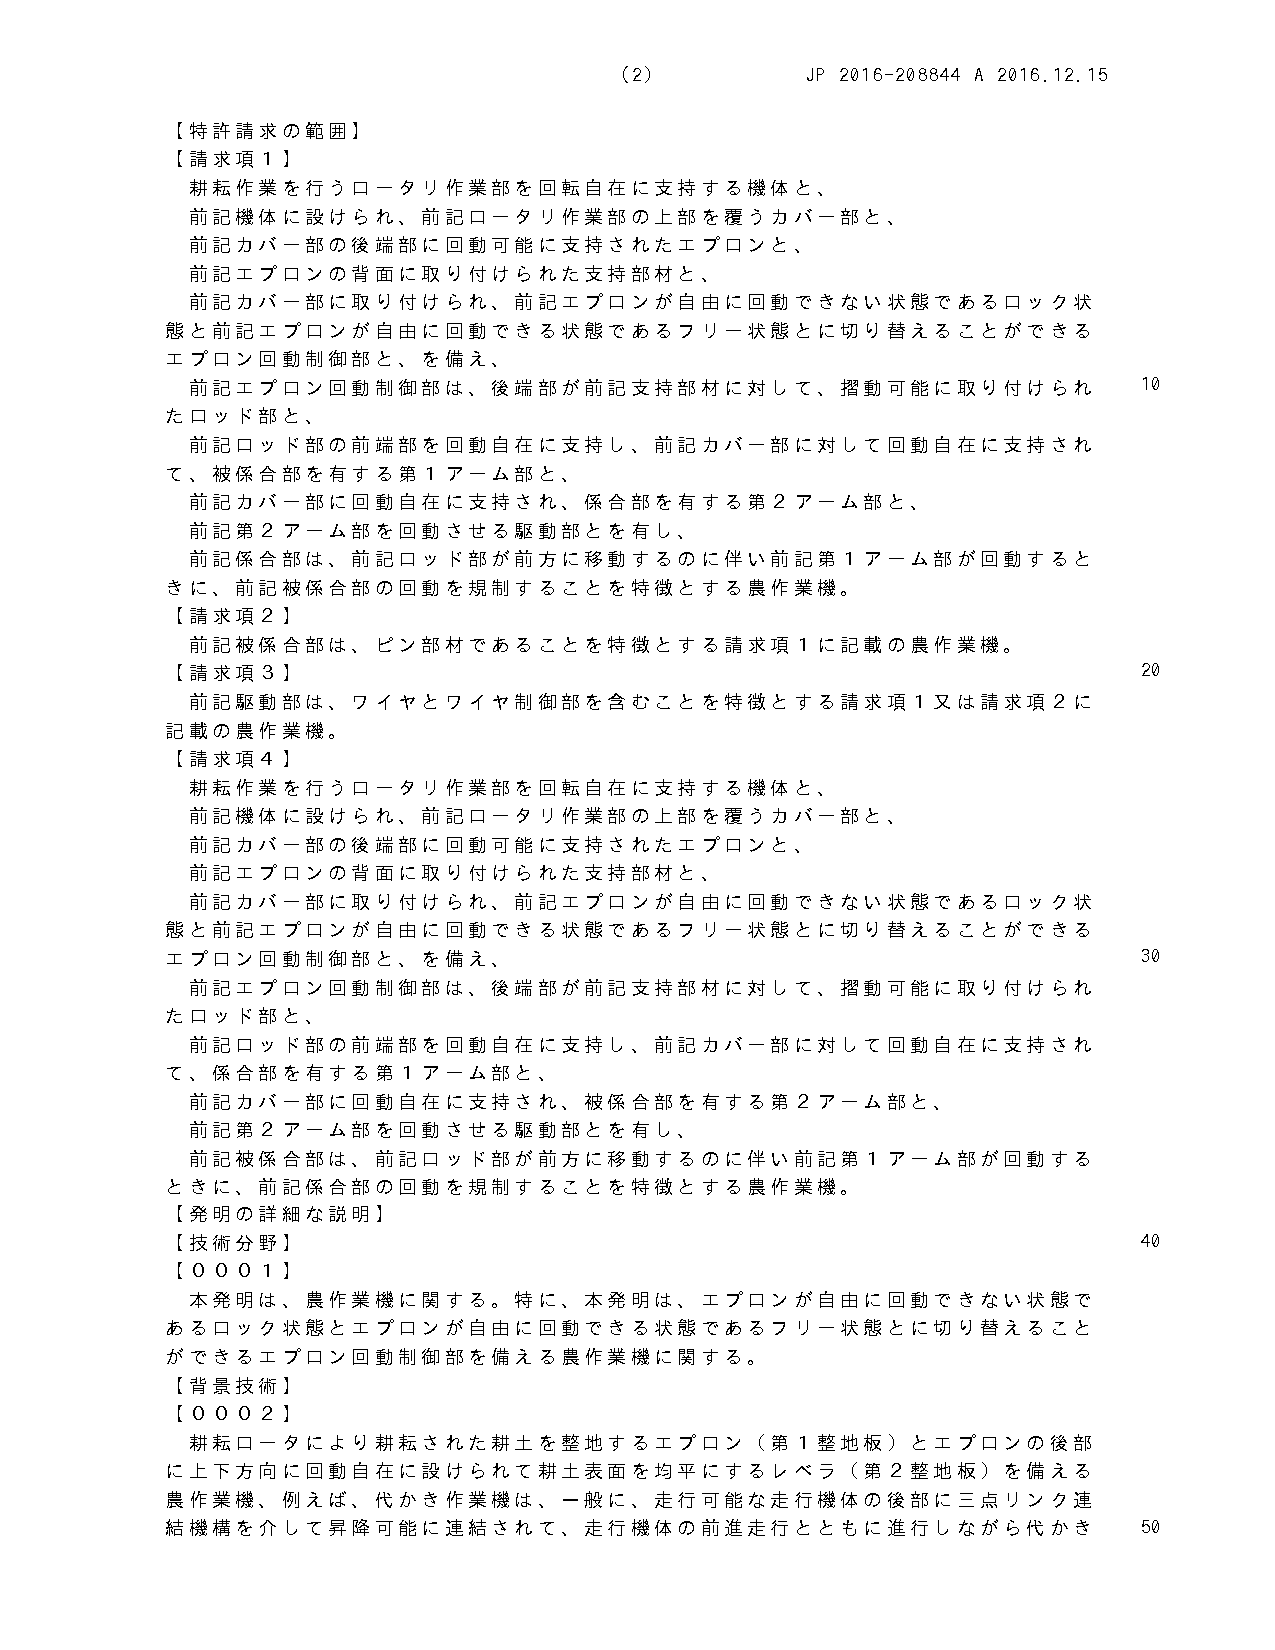
\includegraphics[width=0.55\textwidth,natwidth=500,natheight=1100]{ex1-2.pdf}
  \end{tabular}
  \caption{特許文章例}
  \label{fig:exp}
 \end{figure}

 図\ref{fig:exp}は特許文章の例である.
 発明の範囲を正確に記載するように請求項は普段に使わない学術用語を用いる. また,一般的な文章は単語をなるべく重複しないようにする一方,特許文章は単語を全体を通じて統一して使用し,指示代名詞はなるべく用いず.そのため,特許データベースでは一般的なウェブ文章データベースより多くの単語がある.
 
 \section{特許分類}
 特許では人手によって分類され,特定の分類コードを付いている.
%特許分類を用いることより検索する特許文章が減り,似たようなキーワードを含むが分類が違う特許文章を排除することができる.
 今最も使われている特許分類が世界知的所有権機関(WIPO)による管理されている国際特許分類(IPC)である.
 IPCは世界標準であるため,同じ分類コードが付いているどの国の特許も同じ分類に属する.
 国際特許分類は階層構造であり,一番上の階層はAからHまでの8個のセクションである.
 セクション以下は表\ref{tab:IPC}に表したように四つの階層に分類されている.
 
 \begin{table}[!hbp]
 \center
 \begin{tabular}{cc}
    セクション:A & 健康および娯楽 \\
    サブセクション : 61 & 医学または獣医学:衛生学 \\
    クラス: C & 歯科:口腔または歯科衛生 \\
    メイングループ:5 & 歯の充填または被覆 \\
    サブグループ:08 & 歯冠:その製造;口中での歯冠固定 \\
 \end{tabular}
 \caption{国際特許分類例:A61C 5/08}
 \label{tab:IPC}
 \end{table}
 
 一般に,1つの特許が複数の分類に属する.
 本論文で用いる特許データベースでは一件あたり個の2.4個の分類コードが付いている.
 本論文では特許発明の主体を表す筆頭コードをその特許が属する分類とする.
 
 \section{特許検索}
 特許データベースにおける検索は技術水準調査,新規性調査,侵害調査に分けられる.
 表\ref{tab:type}では3つの検索タイプーを検索対象あるいは検索質問の発端となるものと検索の目的を示す.
 本論文では特許の新規性調査における検索質問の安全性について分析する.
 新規性調査はまだ出願していない発明について検索するため,
 質問意図が漏れたら,
 自社の研究開発動向など企業秘密が知られ,
 特許を攻撃者に先に出願される恐れがある.
 
 \begin{table}[!hbp]
 \center
 \begin{tabular}{|c|c|c|}
 \noalign{\hrule height 1pt}
 検索タイプー & 検索対象(specification) & 検索目的 \\
 \hline
 \tabincell{c}{技術水準調査\\(State of the Art Search)} & イデア & 自分の発明に関連する背景知識を得る \\
 \tabincell{c}{新規性調査\\(Novelty Search)} & 特許願書 & 特許登録の可能性を判断する \\
 \tabincell{c}{無効資料調査\\(invalidity Search)} & 特定な特許 & 特許発明の特許性の有無特許性の有無 \\
 \tabincell{c}{侵害調査\\(Infringement Search)} &  \tabincell{c}{商品と\\商品に関連する技術} & 権利侵害とならないかを判断する \\
 \noalign{\hrule height 1pt}
 \end{tabular}
 \caption{特許検索タイプー}
 \label{tab:type}
 \end{table}

 本論文ではNTCIR-6\cite{NTCIR6}の特許文書集合と無効資料検索タスクの質問を用いて評価実験をする.
 無効資料調査の目的は第三者の発明に特許性がないことを示す根拠となる文章を検索することであるが,
 特定発明の特許性の有無を判断することは新規性調査と一致であるため,
 無効資料検索タスクの質問を新規性調査の質問とすることが妥当であると考えられる.
 


 \chapter{曖昧化検索} \label{s:OBS}
 曖昧化検索は質問者が検索したい真の質問と質問者側で生成したダミー質問を一緒に検索サーバーに提出し,真の質問がどれかを曖昧化するものである.
 本論文では以下のモデル\cite{}を用いて既存な曖昧化検索メカニズムを分析する.
 質問者Aliceがとある検索サーパーに質問を出して手に入れたい情報を検索し,
 検索サーバーが semi-honest な攻撃者であることを仮定する.
 
 質問が単語の集合であり,質問の定義域を単語集合の冪集合にする.
 
 \begin{defi}{ユニバーサル質問集合$Q$.}
  $W$を全ての単語の集合とする.
  ユニバーサル質問集合$Q$とは$W$の冪集合である,つまり
  \begin{equation}
  Q = P(W) = \{A|A \subset W\}
  \end{equation}
 \end{defi}
 Aliceのプロフィールを多項分布と仮定し,Aliceが持つ真のプロフィールを$X$とする.
 
 \begin{defi}{質問者のプロフィール$X$.}
  $T$を全てのトピックの集合とする.
  質問者のプロフィール$X$とは
  \begin{equation}
   X = \{x_i| i \in T\}
  \end{equation}
  $x_i$は質問者がトピック$i$に対して持つ興味の強さを表す.
 \end{defi}
 曖昧化検索メカニズムはAliceのコンピュータで実行する.
 曖昧化検索メカニズムが意味分析ツール$SA$を用いて真の質問$q_R$を分析しダミー質問$q_D$を生成する.
 生成したしダミー質問$q_D$と真の質問$q_R$を1つの質問グループにし,検索サーバーに提出する.
 質問$q$とトピック$t$の関係を表す関数は以下のように定義する,
 
 \begin{defi}{質問-トピックスコア関数:$rscore_{SA}$.}
  $T$を全てのトピックの集合とする.
  質問$q$とトピック$t$の関係を表す関数とは
  \begin{equation}
   rscore_{SA}:Q \times T \to \mathbb{R}
  \end{equation}
 \end{defi}

 \begin{defi}{質問$q$のメイントピック:$\delta_{SA}(q)$.}
  $T$を全てのトピックの集合とする.
  質問$q$のメイントピック$\delta_q$とは
  \begin{equation}
   \delta_{SA}(q) = \argmax_{t \in T} rscore_{SA}(q,t)
  \end{equation}
 \end{defi}

 次は質問$q$のトピックベクトルを定義する.
 質問$q$のトピックベクトル$ttvec_{SA}(q) = (rscore_{SA}(q,t_1 ), \dots , rscore_{SA}(q,t_{|T|})$とは
 $q$と全てのトピック$t_i$の質問-トピックスコア関数$rscore(q, t_i)$を要素として持つ$|T|$次元ベクトルである.
 質問のトピックベクトルを使って質問間の関係を評価することができる.

 検索サーバーがAliceからもらった質問をすべて記録し,その質問たちを分析し得るプロフィールを$Y$にする.

 \begin{defi}{質問比較関数:$C$.}
  質問比較関数$C:Q \times Q \rightarrow \mathbb{R}$を以下のように定義する
  \begin{equation}
  C_{SA}(q_1,q_2) = \frac{(tvec_{SA}(q_1) \cdot tvec_{SA}(q_1))}{||q_1|| ||q_2||}
  \end{equation}
 \end{defi}
 
 
 曖昧化検索は3つ違うレベルな目標がある.
 まずは質問そのものの曖昧化である.
 質問者が検索した真の質問$q_R$はどの質問であるかをわからないようにする.
 2つ目は質問意図の曖昧化である.
 質問者が検索したいものは何であるかをわからないようにする.
 最後は質問者のプロフィール$X$の曖昧化である.
 $Y$から質問者が興味を持つトピックは何であるかをわからないようにする.
 
 質問の曖昧化ができたとしても質問意図の曖昧化ができると限れない.
 {林檎}と{リンゴ}の2つ質問から真の質問を確定することができないが,質問者が林檎について検索したいことが確定できる.
 同じように{林檎}と{梨}の2つ質問から質問者が検索したいを確定することができないが,質問者が果物に興味を持つことが確定できる.
 本論文では質問意図の曖昧化をメインにする.

 次に検索質問のプライバシー保護の代表的な手法,
 否認可能検索(PDS)\cite{providing2009},
 質問者のプライバシーを保護する質問加工法(ETSQ)\cite{embellishing2010},
 質問意図を曖昧化するキーワード検索(HDGA)\cite{masking2014}を紹介する.
 
 \section{否認可能検索}\label{s:PDS}
 否認可能検索という概念を提出したのは\cite{}である.
 つまり, サーバーは特定なユーザーが特定の時間に提出した一連の質問$L = {q_1, q_2, \dots , q_K}$のログを持つと仮定する. 
 ログにアクセスしたある人が真の検索質問が$q_i$だと証明したいとき, $L$の中の任意の質問$q_j$が真の質問となる確率が同じ$1/K$だと証明できる.
 以下に否認可能検索を定義する.
 \begin{defi}{$k−$否認可能検索}
 	質問$q$をユーザーが入力した質問とする.ダミー質問生成システム$DGS$が$k$個の質問を含んでいる質問集合$DGS(q_u)=\{q_1, \dots , q_k\}$を出力しサー
	バーに提出する.$DGS(q_u)$が以下の性質を持つなら,$D(q_u)$をPD-質問集合といい,$D$を$k$−否認可能検索という
	\begin{enumerate}
	\item $\exists q_i \in DGS(q_u),q_i$と$q_u$が意味的に近い
	\item $\forall q_j \in DGS(q_u),DGS(q_j) = DGS(q_u)$
	\item $\forall q_j \in DGS(q_u),q_j$が違うトピックに含まれる
	\item $\forall q_j \in DGS(q_u),q_j$が同じような尤もらしさを持つ
	\end{enumerate}
  \end{defi}
 PDSでは事前に文書集合から高頻度な単語と単語ペアをシード質問として抽出し,
 潜在意味分析(LSA)\cite{LSA1990}を用いてシード質問をトピック空間にマップし,
 トピック空間に距離が近いシード質問をクラスタリングして標準質問とPD-質問集合を構築する.
 検索する場合は,ユーザーが検索したい質問の代わり,
 事前に用意した標準質問集合からトピック空間において質問者が検索したい真の質問と最も近い標準質問が属するPD-質問集合をサーバーに提出し,
 サーバーから検索結果を得,質問者側で真の質問を用いて検索結果をフィルタリングする.
 以下でこの流れを具体的に述べる.
 %潜在意味分析の詳細は第\ref{s:sm}章で述べる.
 \subsection{シード単語と標準質問}
 システムが生成した質問は通常は使わない単語の組み合わせを使うことがある.
 攻撃者がこのような質問をダミー質問と判定し、真の質問を特定する可能性があるため,PDSは標準質問とPD-質問集合を事前に構築する.
 そのため,$Q$の中の全ての質問をカバーすることは不可能である.
 PDSの目標は妥当な再現率を得ることであるため,高頻度な単語だけを使うことは適当だと考えられる.
 
 \begin{algorithm}
 \caption{標準質問の構築}
 \begin{algorithmic}[1]
  \Require シード質問集合$S$
  \State $Q_C \Leftarrow \phi$
  \State Kdtreeを構築し$S$の全ての要素を追加する
  \ForAll {$s_i \in s$}
  \State Kdtree を用いて$s_i$と最も近いシード質問$c_1,c_2$を選ぶ
  \State $cquery = s_i \cup c_1 \cup c_2$
  \If {$cquery \notin Q_c$}
  \State $Q_C = Q_C \cup \{cquery\}$
  \EndIf
  \EndFor
  \Ensure 標準質問の集合$Q_C$
 \end{algorithmic}
 \label{a:cq}
 \end{algorithm}

 まず単語・文書行列に頻出パターンマイニング\cite{apriori2010}を用いて
 $\Delta$回以上に表れた単語と連続する単語からなる単語ペアをシード質問として抽出し,トピック空間にマップする.
 シード質問はユーザーの意図を適切に表さないことが多いため,
 PDSでは意味的に近いシード質問をグループにして標準質問にする.
 アルゴリズム\ref{a:cq}ではこの流れを具体的に説明する.
 このステップの計算量は$O(NlogN)$となる.
 ここで$N$はシード質問の数である.

 \subsection{PD-質問集合の構築}
 PD-質問集合を構築するには,トピックは異なるが尤もらしさが近い標準質問を同じ質問集合に集めれば良い.
 そのため,多様性と尤もらしさを計算する方法を提案する必要がある.
 多様度ではトピック空間の中の距離で評価する.
 人間が作った質問と比較するため,合理的な大きさを持つ質問ログ$Q_L = \{q: q \in Q\}$にアクセスできると仮定する.
 $Q_C$と同様に$Q_L$もトピック空間にマップし,標準質問の近傍の中の$Q_L$の要素数で標準質問の尤もらしさを計算する.
 近傍に多くの$Q_L$に含まれる質問がある標準質問を尤もらしさが高いとする.

 次は3つの部分の和となる標準質問間の関係を評価する関数を定義する.
 質問$q_1$と質問$q_2$のユークリッド距離$edist(q_1,q_2)a$とは,
 \begin{equation}
 edist(q_1,q_2) = \sqrt{\sum_{i \in T}(tvec_{LSA}(q_1)[i] - tvec_{LSA}(q_2)[i])^2}
 \end{equation}
 である.
 ユークリッド距離が遠い質問が異なるトピックに含まれると考えられる.
 質問$q$の強度とは,
 \begin{equation}
 ||q|| = \sqrt{\sum_{i \in T}(tvec_{LSA}(q)[i])^2}
 \end{equation}
 である.
 質問$q$の近傍中の質問数$nhc(q)$とは,
 \begin{equation}
 nhc(q) = count(tvec_{LSA}(q),Q_L,HCUBE(tvec_{LSA}(q),\vec(\delta)))
 \end{equation}
 である.
 ここで$Q_L$は質問ログ,$HCUBE(tvec_{LSA}(q),\vec(\delta))$は$tvec_{LSA}(q)[i] \pm \delta[i]$となる超立方体である.
 $nhc(q)$は超立方体中で$Q_L$に属するベクトルの数を返す.
 
 \begin{defi}{質問間の評価関数:$dis$.}
  \begin{equation}
  	dis(q_1,q_2) = (1 - \frac{edist(q_1,q_2)}{\alpha}) + \frac{|||q_1|| - ||q_2|| |}{\beta} + \frac{|nhc(q_1) -nhc(q_2)|}{\gamma}
  \end{equation}
  ここで,$\alpha$は$Q_C$に属する全ての質問ペア間の最大のユークリッド距離,
  $\beta$は質問ペア間の最大の強度差で,
  $gamma$は質問ペア間の最大の近傍中の質問数の差である.
 \end{defi}
 
 したがって,近傍中の質問数と強度の差が小さく,
 トピック空間中の距離が遠い質問ペアの評価関数の値が低くなり,
 一つのPD-質問集合に入れるべきである.

 次では,質問集合間の評価関数を定義する.
 $A = {a_1, \dots , a_n}$と$B = {b_1 , \dots , b_m}$を2つ質問集合とする.
 $A$,$B$間の評価関数とは,
 \begin{equation}
    dis(A,B) = (1 - \alpha_1 / \alpha) + \beta_1 / \beta + \gamma_1 \gamma
 \end{equation}
 である.
 ここで,$\alpha_1 = \min_{i,j}(edist(a_i,b_j))$は2つの質問集合に属する質問ペア間のユークリッド距離の最小値であり,
 $\beta_1 = |\frac{\sum_i||a_i||}{n} - \frac{\sum_j||b_j||}{m}|$と
 $\gamma_1 = |\frac{\sum_inhc(a_i)}{n} - \frac{\sum_jnhc(b_j)}{m}|$は質問集合の強度と近傍中の質問数の平均数の差である.
 
 \subsection{凝集型クラスタリング}
 PDSでは,まず質問ペアを要素とするレベル1集合$L_1$を生成する.
 $Q_C$に属する全の質問ペア間の評価関数の値の行列を計算し,
 評価関数の値が小さいから大きい順で質問ペアを$L_1$に加える.
 質問ペア$(q_i,q_j)$に対し,$q_i$か$q_j$ は評価関数の値がもっと小さいペアに属する可能性がある.
 その場合,$q_i$か$q_j$がすでに$L_1$にあることとなり,次に評価関数の値が小さいな質問ペアを選ぶ.
 選んだ質問ペアをマージし,次のレベルの集合($L_2$,$L_3$,etc)を作る.
 マージステップはレベル変数$l$が$log_2k$になるまで続ける.
 したがって,最終レベルの集合中の質問クラスターの大きさが$k$となり,オーバーラップがないと保証する.

 \subsection{PD-質問集合の使用}
 ユーザー質問$q_u$に近い標準質問を探すため,
 $q_u$を意味区間にマップし,
 $C(q_u,q_c)$が一番大きい標準質問$q_c$を選び,
 $q_c$が属するPD-質問集合をサーバーに提出し,
 クライエント側でユーザー質問を用いて検索結果をフィルターする.
 一定な再現率を得るため,普段の検索より多くの文書を手に入れる必要があるが,フィルターステップがこの影響をなくす.

 ユーザー質問の全ての単語がPD-質問集合を構築するために使った単語リストに含んでいないなら,
 ユーザー質問を意味区間にマップすることは不可能である.
 しかし,単語量が十分大きいなら,そのような状況を発生する可能性は低いと考えられる.
 また,(十分大きな)単語リストに含んでいない単語はユーザーの意図を漏洩するリスクが高い.
 ユーザーがそのような質問を提出したとき,ユーザーに危険性を警告し,検索しないようにすることが考えられる.

 \section{質問者のプライバシーを保護する質問加工法} \label{s:ETSQ}
 今テキスト検索エンジンの大半が類似検索である.
 全ての質問単語を含んでいる文章しか検索できないキーワード検索と違い,
 類似検索は文章と質問の関連性を計算し文章にスコアをつける\cite{if2006}.
 毎回全ての文章との 関連性を計算しないために,
 検索エンジンが単語と文章の類似度を転置ファイルに保存し,
 質問の単語と文章の類似度の和を質問とその文章の関連性とする.
 このような計算が必要であるため,\cite{pss2006,opf2005,pke2004,soe2000}などキーワード検索しか対応できない研究は類似検索に応用できない.

 PDSをはじめに多くの曖昧化検索メカニズム\cite{masking2014,praw2005,goo2009}は質問の全体を分析し,適切な$K−1$個のダミー質問を選ぶ.
 質問の全体ではなく単語ごとにダミー単語を混ぜれば,
 真の質問である可能性がある質問数が増え,攻撃者が真の質問を見破る確率が下がる.
 質問者がいつのトピックに対して検索するとき,一つの単語を複数回使うと考えられる.
 毎回違うダミー単語を混ぜると同じ質問者の質問に出る頻度が高い単語が真の質問単語となる可能性が頻度が低い単語より大きくなる.
 そんなリスクを防ぐためETSQは単語バケットを事前に作り,真の質問単語と同じバケットにある他の単語をダミー単語とする.
 また,単語ごとダミーを混ぜるため長い質問と類似検索に対応できる.

 \subsection{類似検索}
 コーパス$D$における検索エンジンが質問を処理するとき基本的には転置ファイルを用いている.
 転置フィルは質問単語の集合$W$と全ての単語の転置リストからなる.
 単語$w_i \in W$の転置リスト$L_i$が$\langle d_i,p_{ij}\rangle$の列である.
 $p_{ij \in \Re}$は単語$t_i$と文>章$d_i \in \mathcal{D}$の関連性である.
 $t_i$が$d_i$に現れたなら$p_{ij}$の値は$0$より大きい,現れなかったなら$0$となる.
 空間圧縮のために$p_{ij}=0$な$d_i$は$L_i$に含まれていない.

 質問$q=\{w_i\}$と文章$d_i$と関連性は以下のように計算する
 \begin{equation}
 Score_{d_j,q} = \sum_{w_i \in q}p_{ij}
 \end{equation}
 したがって転置リスト$L_i$に含まれている文章だけが$0$以上のスコアを持ち,$q$と関連があると見なす.
 転置フィルを全体暗号化しても,サーバーは転置リストの長さとアクセス頻度などの情報から真の関係値を推定できるため,
 そのような方法は無意味だと考えられる.
 
 \subsection{単語バケツ} 
 本節では単語バケツを作る方法を述べる.
 まずアルゴリズム\ref{a:bkt}を用いてWordNetデータベース中の意味的近い単語を隣にして全ての単語一列に並べる.
 リンクが多いsynsetが意味的に豊富であるため,単語を一列に繋がる種として使われ,synsetの関係数が多い方から小さい方への順で処理する.
 複数の意味を持つ単語が属するsynsetが意味的近いと考え,同じ単語を持つsynsetを隣に並べる.
 また反意関係,上位下位関係,全体部分関係を持つsynsetを隣に並べる.
 2つの操作により,列に近い単語の意味も近いと保証する.

 WordNetデータベースにアルゴリズム1を行った結果データベース中全ての$117,798$個の名詞を一列に並べ,アルゴリズムに有効性を証明した.

 \subsection{バケツ作り}
 \begin{algorithm}
 \caption{単語を一列に並べる}
 \begin{algorithmic}[1]
 \Function{ProcessSynset}{synset ss}
  \If {$ss$の単語が複数の既存な単語列に含まれている}
   \State そんな単語列を結合する
   \State 結合した単語列を$sq$にする
  \ElsIf {$ss$の単語が既存な単語列に含まれていない}
   \State 新たの単語列を作る
  \Else {\, $ss$の単語の一つが一つ既存な単語列に含まれている}
   \State その単語列を$sq$にする
  \EndIf
  \State 処理していない$ss$の単語を$sq$に加える
  \State $ss$の単語を処理したとマークする
  \State $ss$を処理したとマークする
  \State 単語列$sq$を返す 
 \EndFunction
 \Function{SequenceVocab}{WordNet wndb}
  \State 全てのsynsetを関係数が多い方から小さい方への順で並べる
  \State 全てのsynsetを処理していないとマークする
  \State 全ての単語を処理していないとマークする
  \State $SeqSet = \phi$
  \ForAll {処理していないsynset $ss$}
   \State $sq=ProcessSynset(ss)$;$sq$を$SeqSet$に加える
   \ForAll {$ss$と反意関係,上位下位関係,全体部分関係をもつsynset $ss'$}
    \State 処理していない$ss'$の単語を$sq$に加える
    \State $ss'$の単語を処理したとマークする
    \State $sq=ProcessSynset(ss')$;$sq$を$SeqSet$に加える 
   \EndFor
  \EndFor
 \EndFunction
 \end{algorithmic}
 \label{a:bkt}
 \end{algorithm}

 \begin{figure}[!hbp]
  \centering
  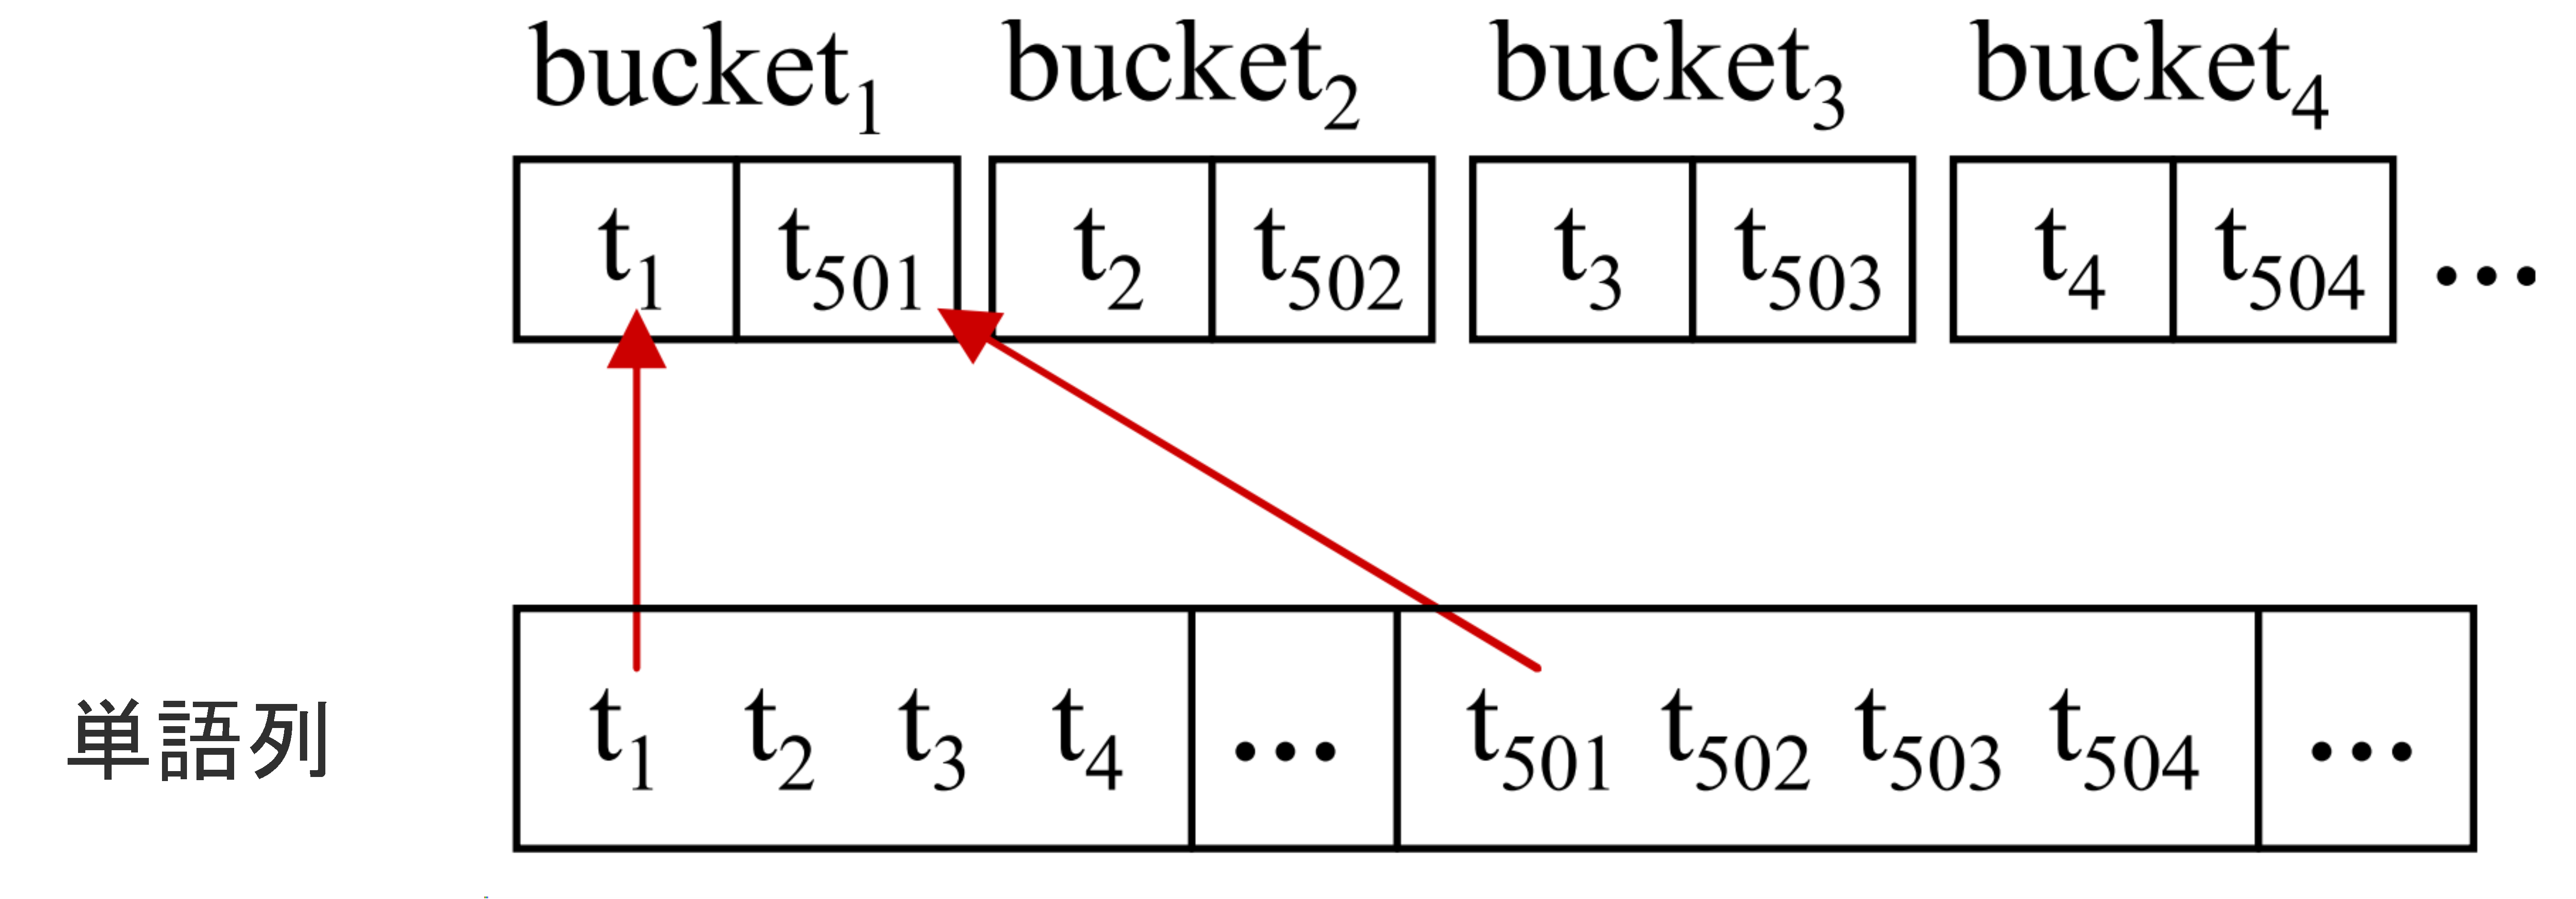
\includegraphics[width=0.8\textwidth,natwidth=5677,natheight=1982]{rk11.png}
  \caption{バケツ作り-$N=1000,BktSz=2$}\label{fig:bkt}
 \end{figure}

 \begin{algorithm}
 \caption{単語列から単語バケツを作る}
 \begin{algorithmic}[1]
 \Function{GenerateBuckets}{sq,BktSz,Segsz}
  \State $N=$単語列$sq$の長さ
  \State $\#Seg=N/SegSz$
  \State $sq$を同じ長さのセグメントに分割する$S_1,S_2, \dots , S_{\#Seg}$
  \State セグメント中の単語を特殊レベルが大きい方から小さい方への順で再配列する
  \For {$i = 1 to N/(BktSz * SegSz)$}
   \State ActiveSeg = $\phi$
   \For {$j = 1 to BktSz$}
    \State $ActiveSeg = ActiveSeg \cup S_{(j-1)N/(BktSz * SegSz)}$
   \EndFor
   \For {$j = 1 to SegSz$}
    \State 新たなバケツ$B=\phi$を作る
    \State ActiveSeg中の全てのセグメントの$j$番目の単語を$B$に入れる
    \State $B$を出力する
   \EndFor
  \EndFor
 \EndFunction
 \end{algorithmic}
 \label{a:bkt2}
 \end{algorithm}
 
 次ではアルゴリズム\ref{a:bkt}で出力した単語列を単語バケツにする.
 アルゴリズム2がその過程を表している.
 バケツの大きさを$1 \leq$BktSz$\leq N$に設定する.
 バケツの数が\#Bkts$=N/$BktSzである.
 同じバケツ中の単語を可能な限りに違う意味にするために単語列の
 $1,\#$BktSz$+1,2*\#$BktSz$+1, \dots,($BktSz$-1)*\#$BktSz$+1$番目の単語をバケツ$1$に,
 $2,\#$BktSz$+2,2*\#$BktSz$+2, \dots,($BktSz$-1)*\#$BktSz$+2$をバケツ$2$に,
 $i,\#$BktSz$+i,2*\#$BktSz$+i, \dots,($BktSz$-1)*\#$BktSz$+i$をバケツ$i$に入れる.
 図\ref{fig:bkt}が$N=1000,BktSz=2$のときのバケツ作り過程を表している.
 その操作により,2つのバケツ$i$と$j$の同じ位置の単語間の距離が同じ$\|i-j\|$であり,意味的な距離の差も小さいと考えられる.
 またバケツ同じ位置の単語間の距離が違う位置の単語間の距離より近いため、真の質門の単語が同じ位置にあると仮定する。
 したがって,真の質問の単語が意味的に近いときあるいは一つのトピックに集中したとき,
 バケツの中のダミー単語も同じように一つのトピックに集中すると考えられる.
 しかし,バケツ中の単語の特殊レベルがランダムであり,大きく違う可能性がある.

 バケツ中の単語の特殊レベルを調整するために,隣接のバケツ間の単語交換を行う.
 実践的には単語を単語バケツに配置する前に単語列を同じ長さSegSz$\leq N/$BktSzのセグメントに分割し,
 セグメント内の単語を特殊レベルが大きい方から小さい方への順で再配列する.
 SegSzがBktSzの整数倍である必要がある.
 図\ref{fig:bkt2}が図\ref{fig:bkt}の上に単語列の再配列を加えた流れを表している.
 その結果,同じバケツにある単語のセグメント内の順番が同一であり,特殊レベルが近くなると考えられる.

 \begin{figure}
  \centering
  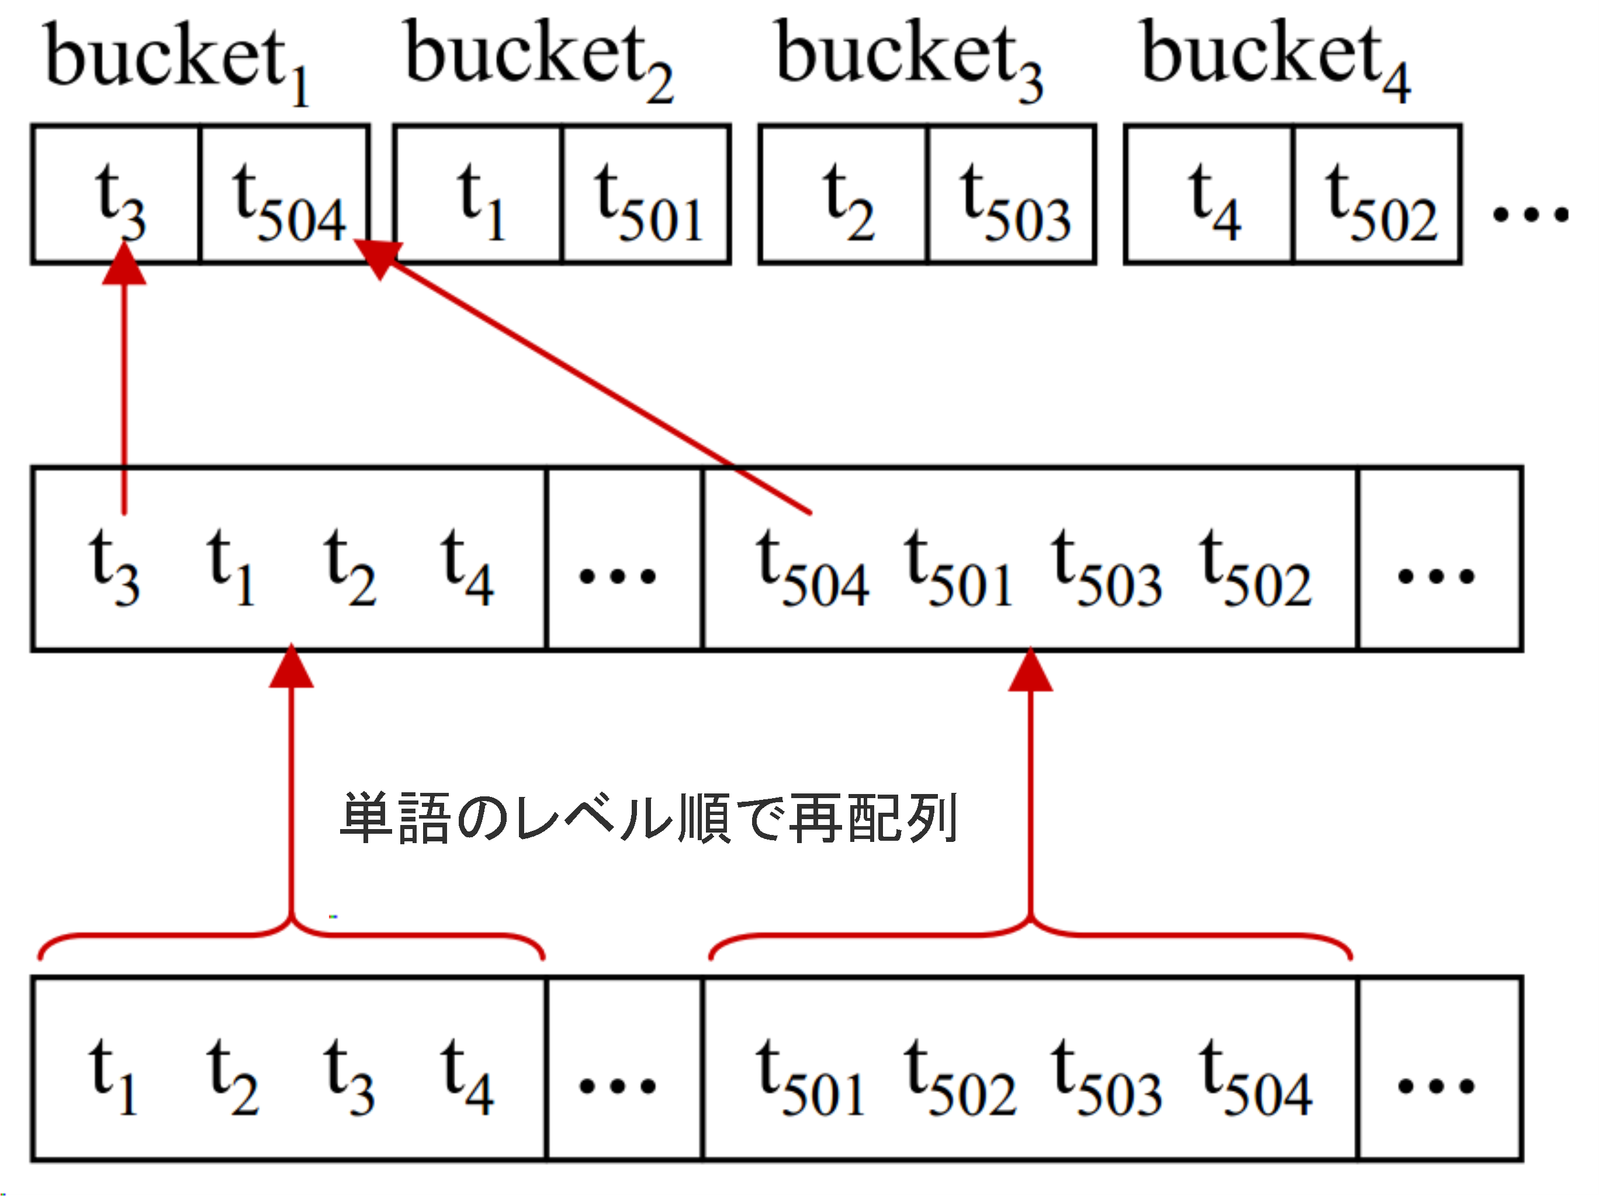
\includegraphics[width=0.5\textwidth,height=0.3\textwidth,natwidth=1600,natheight=1196]{rk13.png}
  \caption{バケツ作り-$N=1000,BktSz=2,SegSz=4$}\label{fig:bkt2}
 \end{figure}

 バケツ作りには2つのパラメータを設定する必要ある.
 SegSzが2つのリスクのトレードオフとなる.
 SegSzが増加することは単語交換を行う範囲が増大することに相当する.
 SegSzが大きければ大きいほどバケツ中の単語の特殊レベルが近くなる.
 一方、単語間の意味的な距離も近くなる可能性がある.
 もう一つのパラメータBktSzがプライバシーと計算時間のトレードオフとなる.
 BktSzが大きくなると,真の質問を特定する可能性が下がるが,検索エンジンが処理する質問単語が増加する.
 
 \subsection{プライベート検索スキーム}
 本節では真の質問単語だけの関連性スコアを計算できる検索スキームを述べる.
 検索スキームは質問加工,質問検索と結果処理三部分からなる.

 \begin{algorithm}
 \caption{質問加工}
 \begin{algorithmic}[1]
 \Function{GenerateBuckets}{sq,BktSz,Segsz}
  \Require 真の質問単語$t_i$の集合
  \Ensure 加工した質問$q$
  \ForAll {真の質問単語$t_i$}
   \State Bkt$=t_i$が属する単語バケツ
   \ForAll {$t_j \in $Bkt}
    \If {$t_i == t_j$} $\mu_j=1$
    \Else $\,\mu_j=0$
    \EndIf
    \State $E(u_j) = g^{\mu_j}\mu^r$
    \State $\langle t_j,E(\mu_j)\rangle$を$q$に入れる
   \EndFor
  \EndFor
 \EndFunction
 \end{algorithmic}
 \label{a:qe}
 \end{algorithm}

 アルゴリズム\ref{a:qe}が質問加工の流れを表す.
 真の質問単語が属するバケツの中の他の単語を全てデミー単語として質問に加える.
 デミーを加えた質問の単語$t_j$に$E(\mu_j)$を付け,$t_j$が真の質問単語なら$\mu_j=1$,ダミー単語なら$\mu_j=0$.
 $E(\cdot)$は加算可能な準同型暗号\cite{benaloh_dense_1994}の暗号化関数である.
 加算可能な準同型暗号が以下2つの特徴を持つ.
 二つの暗号文$E(m_1), E(m_2)$が与えられた時に,平文や秘密鍵なしで$E( m_1 + m_2 )$を計算できる.
 また,同じメッセージ$m$が複数の暗号文に対応でき,攻撃者が暗号文の頻度から$m$を推定することを防げる.

 \begin{algorithm}
 \caption{質問検索}
 \begin{algorithmic}[1]
 \Function{GenerateBuckets}{sq,BktSz,Segsz}
  \Require 加工した質問$q$
  \Ensure 文章とその文章暗号文した関連性スコアの集合$R$
  \State $R=\phi$
  \ForAll {$\langle t_i,E(\mu_i)\rangle \in q$}
   \ForAll {$\langle d_j,p_{ij}\rangle \in L_i$}
    \If {$\exists \langle d_j,E(score_j)\rangle \in R$}
     \State $E(score_j)=E(score_j)*E(\mu_j)^{p_{ij}}$
    \Else
     \State $\langle t_j,E(\mu_j)^{p_{ij}}\rangle$を$R$に入れる
    \EndIf
   \EndFor
  \EndFor
 \EndFunction
 \end{algorithmic}
 \label{a:qs}
 \end{algorithm}

 アルゴリズム\ref{a:qs}がサーバー側の検索過程を表す.
 サーバーが単語と文章の関連値を保存している転置フィルを用いて文章の関連性スコアを計算する.
 加算可能な準同型暗号の特徴より,$E(\mu_j)^{p_{ij}}=E(\mu_j*p_{ij})$.
 $t_j$がダミー単語であれば,$E(score_j)*E(\mu_j)^{p_{ij}}=E(score_j)*E(0*p_{ij})=E(score_j)$.
 復号した関連性スコアには影響を与えない.
 したがって,$score_j$が真の質問単語と文章の関連値$p_{ij}$の和となる.

 最後に質問者がサーバーがらもらった結果集合の関連性スコアを復号し,
 その値を用いて文章を再配列するとプライバシー保護手法を使っていない検索エンジンと同様な検索結果がもらえる.

 \section{質問意図を曖昧化するキーワード検索}

 HDGAは\cite{toi2012}提案した潜在的ディリクレ配分法(LDA)\cite{lda2003}に基づく質問意図の曖昧化メカニズム(TIO)の改良手法である.
 LDAの詳細は第\ref{s:sm}章で述べる.
 HDGAが以下の特徴を持つ,
 まず,サーバーに提出した質問グループに属する各質問が違うトピックに属し,ダミー質問の生成過程が相互独立である.

 次に,HDGAはTIOのように真の質問をカバーできるトピックからダミー質問を作るではなく
 同じ質問グループに属する質問が同じ地位を持つ.

 そして,HDGAがハッシュ関数Highest Random Weigh(HRW)\cite{hrw1998}を用いてダミートピックを選び,トピックの出現頻度を均一にする.

 \begin{algorithm}
 \caption{HDGA(On Masking Topical Intent in Keyword Search)}
 \begin{algorithmic}[1]
  \Require 質問:$q_1$
  \State $Q = \{q_1\}\delta_{q_1} = \argmax_{t \in T} Pr[t|q_1]$
  \ForAll {$t \in T \setminus \{\delta_{q_1}\}$}
  \State $e_t = h(\delta_{q_1}||t||s)$
  \EndFor
  \State $T_D = \{t^1_{q1},t^2_{q1}, \dots , t^2_{q1} | \forall t_1 \ \in T_D , \forall t_2 \ \in T \setminus T_D, e_{t_1} > e_{t_2} \}$
  \ForAll {$t \in T_D $}
  \While { $ \argmax_{t \in T} Pr[t|q'] \neq t$}
  \State $Pr[w|t]$に基づいて$|q_1|$個の単語をランダムに選び,ダミー質問$q'$を作る
  \EndWhile
  \State $Q = Q \cup \{q'\}$
  \EndFor 
  \State $Q$をシャッフルする
  \Ensure $Q$
 \end{algorithmic}
 \label{a:HDGA}
 \end{algorithm}

 アルゴリズム\ref{a:HDGA}がHDGAの質問生成メカニズムを表す.
 ここで$Pt[w|t]$がLDA分析の結果であり,$h$がHRWハッシュ関数である.

 \chapter{意味分析} \label{s:sm}
 第\ref{s:OBS}章で述べたように質問意図を隠せるダミー質問を作るために
 質問が持つ意味を計算機に理解させなければならない.
 まず,文章や質問などをベクトルで表す必要がある.
 自然言語研究で多く使用されるベクトル表現方法がbag-of-wordsである.
 bag-of-wordsとは単語を袋に入れるように,単語の出現順番などの情報を捨て,
 単語の出現頻度だけをベクトル要素とする表現方法である.
 次に質問が持つ意味を数字にすると,
 質問をトピックベクトルで表現できる.
 したがって,質問が持つ意味を数字にすることは
 質問を記述するために必要な次元数を減らすことであると考えられる.
 情報検索分野ではコーパス中の文章を記述するために必要な次元数を減らす研究を進めている.

 $tf\text{-}idf$はが単語とコーパス中の文章の関連性を実数値で表せるため,
 文章数$|D| \times$単語数$|W|$の行列$M$でコーパスを記述できる.
 潜在的意味解析(LSA)は行列$M$を特異値分解(SVD)し低ランク近似し,より高い圧縮を得る.
 しかし,LSAモデルのパラメータ数がコーパス中の文章数の共に増加するためオーバーフィットの恐れがあり,
 コーパスに含まれていない文章を記述する方法が明らかにさせていない.
 そのような問題を解決するために確率モデルである潜在的ディリクレ配分法(LDA)が提案された.

 本論文ではこの3つの意味分析手法を全て用い,
 評価実験をする.
 以下では上記意味分析手法を紹介する.

 \section{tf-idf}
 コーパス中に含まれている文書の集合を$D$とし,
 単語$w_i$の文章$d_j$における出現回数を$n_{i,j}$とする.
 単語$w_i$の文章$d_j$における出現頻度を
 \begin{equation}
 tf_{i,j} = \frac{n_{i,j}}{\sum_k n_{k,j}}
 \end{equation}
 単語$i$の逆文書頻度を
 \begin{equation}
 idf_i = log \frac{|D|}{|d|w_i \in d, d \in D|}
 \end{equation}
 と定義し,
 \begin{equation}
 tfidf_{i,j} = tf_{i,j} \cdot idf_i
 \end{equation}
 によって単語$t_i$の文章$d_j$における$tf\text{-}idf$値を計算する.
 
 本論文では国際特許分類を用い特許データベースに属する文章を$632$個の分類にし,
 各分類をトピックとし,
 \begin{equation}
 tfidf_{i,k} = \sum_{d_j \in t_k}tf_{i,j} \cdot idf_i
 \end{equation}
 によって単語$t_i$のトピック$t_k$における$tf\text{-}idf$値を計算する.
 人手により分類されている国際特許分類をトピックにしたため,
 各トピックの意味が明らかである.

 \section{潜在的意味解析}
 特異値分解(SVD)を用いて単語をトピック空間にマップすることが潜在的意味分析の基礎である.
 LSAではトピック空間中の単語と文書の関係を用いて多義性と同義性の問題を解決する.
 つまり、 綴りが違うが同じような意味を持つ単語はトピック空間での距離が近いようにできる.

 単語$\times$文書行列$M$の$(i,j)$番目の要素は単語$w_i$のが文章$d_j$における$tf\text{-}idf$値である.
 $M$を特異値分解$M = USV^T$し、$U$、$S$、$V$ の各列ベクトルを特異値が大きい順に$K$個用いて$G$の低ランク近似$G_K=U_KS_KV_{K}^T$を得る.
 このように低ランク分解によって、単語とトピックの関係を分析できる.
 $M_K$の$(i,j)$番目の要素は$i$番目の単語と$j$番目のトピックの関係を表す.
 その値が大きければ大きいほど単語とピックの関係が強い.
 単語$w_i$と対応する行列$M_K$の行$\ell_i$を単語$w_i$のトピックベクトルとし,
 \begin{equation}
 rscore_{LSA}(q,t_j) = \sum_{w_i \in q}\ell_i[j]
 \end{equation}
 によって質問$q$とトピック$t_j$の関連性を計算する.
 
 本論文では単語$\times$文書行列$M$の代わりに単語$\times$国際特許分類行列$M'$を用いる.
 単語$\times$国際特許分類行列$M'$の$(i,j)$番目の要素は単語$w_i$の国際特許分類$t_k$における$tf\text{-}idf$値である.
 国際特許分類は特許データベースの大きさと関係なく一定であるため,
 文章数の増加によるオーバーフィットを防ぐ.

 \section{潜在的ディリクレ配分法}
 潜在的ディリクレ配分法(LDA)は文章の確率生成モデルである.
 LDAでは文章が複数の潜在的トピックからランダムに生成されると仮定し,
 トピックをそのトピックごとに単語の出現頻度で表す.

 
 LDAではコーパス$D$に含まれている長さが$n_d$である文章$d$の生成過程を以下のように仮定する:
 \begin{itemize}
 \item {\em コーパス$D$における各潜在的トピック$t$を生成する}$\phi_{t} \thicksim Dir(\beta)$
 \item {\em トピック分布ベクトル$\theta_d$を生成する}$theta_d \thicksim Dir(\alpha)$
 \item 各単語$w \in d$に対して:
  \begin{itemize}
   \item {\em $w$が属するトピック$t$を決める}$t \thicksim Mulinomail(\theta_d)$
   \item {\em $w$を決める}$w \thicksim Multinomial(\phi_{t})$
  \end{itemize}
 \end{itemize}
 
 ここで$\alpha,\beta$は$|T|$次元ベクトルで,Dirichlet分布のパラメータであり,
 $\theta_d,\phi_{t}$は確率ベクトルである.

 このグラフィカルモデルを図\ref{fig:LDA}に示す.
 \begin{figure}
 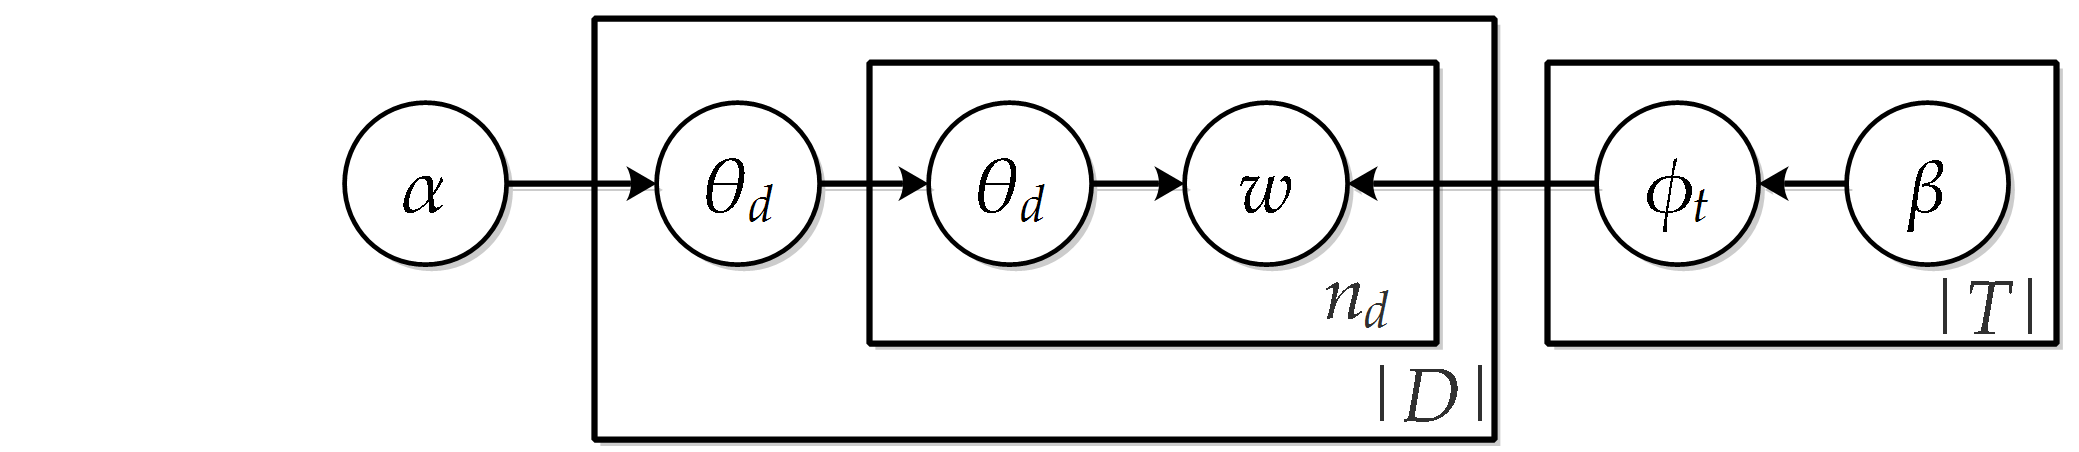
\includegraphics[width=0.9\textwidth,natwidth=557,natheight=141]{LDA.png}
 \caption{LDAのグラフィカルモデル}
 \label{fig:LDA}
 \end{figure}
 
 全ての文章が同じ確率を持つと仮定すると,
 \begin{equation}
 p(t) = \sum_{d \in D}\theta_{d,t}p(d) = \frac{\sum_{d \in D} \theta_{d,t}}{|D|}
 \end{equation}
 によってコーパス$D$の中の各トピックの確率を計算し,
 \begin{equation}
 rscore_{LDA}(q,t) = p(t|q) \thicksim p(q|t)p(t) = \prod_{w \in q}p(w|t)p(t)
 \end{equation}
 によって質問$q$と各トピックの関係性を計算できる.


 \chapter{プライバシー分析(攻撃手法)}
 本論文では攻撃者が質問者が質問意図を隠していること
 と
 質問者が用いている質問曖昧化手法のメカニズムを知っているを前提とし,
 攻撃手法を考える.

 曖昧化検索は3つの違うレベルな目標があると同じように
 曖昧化検索に対する攻撃手法も3つの違うレベルな目標がある.
 ダミー質問が混ぜられた質問グループから真の質問$q_R$を見つかる.
 ダミー質問が混ぜられた質問グループから質問者が検索したいものを見つかる.
 ダミー質問が混ぜられた質問ログから質問者が興味を持つトピックを見つかる.

 1つ目の目標に対して本論文では質問$q$と質問$q$のメイントピック$\delta_{SA}$間の関連性を攻撃するメイントピック攻撃を提案する.
 質問者が検索したいものを定義するのは難しいため,本論文ではダミー質問の検索結果と真の質問の検索結果が一致する割合を用いて評価する.
 そして,3つ目の目標を達成できる既存な攻撃手法類似度攻撃\cite{simattack2016}を紹介し,改良手法を提案する.

 \section{メイントピック攻撃}
 HDGAなど真の質問とダミー質問を1つの質問グループにして提出する曖昧化手法対して,
 ダミー質問が真の質問と同様に全ての単語が1つのトピックに集中することが失敗したら,
 真の質問と真の質問のメイントピックの関連値が
 ダミー質問とダミー質問のメイントピックの関連性より強いと考えられる.
 メインとピック攻撃は1つの質問グループの中で自分のメイントピックとの関連性が一番高い質問を
 真の質問とする.

 また,ETSQは真の質問単語ごとにダミー単語を混ぜ,1つの加工した質問にして提出する.
 関係が強い単語が他のトピックと関係が強い単語の数より多い,
 加工した質問のトピックと真の質問のトピックが一致することが考えられる.
 また,一つのバケツの中の単語が意味的に遠いため,
 ダミー単語が真の質問単語のメイントピックとの関連性が弱いと考えられる.
 メイントピック攻撃では各単語バケツ中質問のメイントピックと一番関連値が強い単語を真の質問の単語と推定する.

% \begin{algorithm}
% \caption{メイントピック攻撃}
% \begin{algorithmic}[1]
%  \Require 質問:$q=\{t_i\},$単語のトピックベクトル集合$L=\{\ell_i\}$
%  \State $R=\phi, \, \ell=0$
%  \State $\ell=\sum_{t_i \in Q}\ell_{t_i}$
%  \State $maintopic = \argmax_j \ell[j]$
%  \ForAll {$bk_k \in q $}
%  \State $R=R \cup \{\max_{t_i}l_{t_i}[maintopic]\}$
%  \EndFor \\
%  \Return $R$
% \end{algorithmic}
% \label{a:mt}
% \end{algorithm}

 \section{類似度攻撃(事前情報あり)}
 類似度攻撃(SimAtt)\cite{simattack2016}は質問者が提出した質問と攻撃者が事前に得た質問者の質問ログ間の類似度を計算し,
 この類似度を用い質問者の新の質問を見破る.
 Simattでは単語ベクトルで質問を表し,
 質問ログを質問の集合とする.
 アルゴリズム\ref{a:simatt}が質問$q$と質問者のログ$P_u$間の類似度$sim_{q,P_u}$の計算方法を示す.

 \begin{algorithm}
 \caption{類似度計算}
 \begin{algorithmic}[1]
  \Require 質問$q$,ユーザープロフィール$P_u$,スムージングパラメータ:$\alpha$
  \For {$q_i \in P_u$}
  \State $coef[i] \leftarrow 2 \cdot |q \cap q_i| \cdot \frac{1}{|q|+|q_i|}$
  \EndFor
  \State $coef \gets sort(coef)$
  \State $sim \gets coef[0]$
  \For {$i \in [1,|P_u|]$}
  \State $sim \gets \alpha \cdot coef[i] + (1 - \alpha) \cdot sim$
  \EndFor
  \Ensure $sim_{q,P_u}$
 \end{algorithmic}
 \label{a:simatt}
 \end{algorithm}

 ここで$coef[i]$は質問$q$と$P_u$に属する質問$q_i$間のDice係数\cite{}で,
 $\alpha$が重み係数である.
  
 \begin{algorithm}
 \caption{SimAtt}
 \begin{algorithmic}[1]
   \Require 質問グループ$G$,ユーザープロフィール$Pu$,スムージングパラメータ:$\alpha$
   \State $q^* = \argmax_{q \in Q}sim_{q,Pu}$
   \Ensure $q^*$
 \end{algorithmic}
 \end{algorithm}

 SimAttは質問グループの中質問者の質問ログと一番類似度が高い質問が真の質問であると判定する.
 攻撃方法は単純であるが,\ref{s:}の実験結果は特許データベースにおける攻撃の強さを示す.

 \section{類似度攻撃2(事前情報なし)}
 攻撃者が事前的に質問者の真の質問ログを持たないとSimAttを用いることができない.
 本節ではダミー質問を混ぜた質問ログのみから真の質問を見つかる攻撃手法SimAtt2を提案する.
 質問者が同じトピックに対して複数の質問を提出することが考えられる.
 PDSなど真の質問と距離が遠い質問をダミー質問にする質問曖昧化手法では
 真の質問は同じトピック$t$に属するとしてもダミー質問は同じように別のトピック$t'$に属すると限れない.
 トピックの出現頻度から真の質問を見つかることができ,
 真の質問間の類似度がダミー質問間の類似度より高いと考えられる.
 ETSQではトピックの出現頻度を均一にできる.
 しかし,ETSQは$Pr(w|t)$に基づいて単語をランダムに選び,ダミー質問を生成するため,
 同じトピックに属するダミー質問間の距離が真の質問間の距離ほど近いと限れない.
 また,真の質問$q_1,q_2$が意味的近いトピック$t_1,t_2$に属するとき,
 ダミー質問$q_1',q_2'$が属するトピック$t_1',t_2'$も意味的近いと保証できない.
 したがって,意味的近い一連の質問が真の質問である可能性が高い.
 本論文では同じ質問者が提出した全ての質問グループから1つ質問を選び出した質問集合を質問列という.
 アルゴリズム\ref{a:simatt2}が意味的近い質問列を取り出す攻撃手法を示す.

 \begin{algorithm}
 \caption{SimAtt2}
 \begin{algorithmic}[1]
  \Require 質問グループ列$\hat{G}=\{ G_1,G_2, \dots , G_m\}$,スムージングパラメータ:$\alpha$
  \For {$j \in |G_1|$}
   \State $\hat{Pu}[j] = G_1[j]$
   \State $\hat{Put}[j] = \Phi$
   \State $d[j] = 0$
  \EndFor
  \For {$i \in [2,m]$}
   \For {$j \in |G_i|$}
   \State $\hat{Put}[j] = \argmax_{Pu \in \hat{Put}}sim_{G_i[j],\hat{Put}[j]}$
   \EndFor
   \State $q^*_i = \argmin_{G_i[j] \in G_i}sim_{G_i[j],\hat{Put}[j]}$
   \For {$j \in |Q_i|$}
    \State $\hat{Pu}[j] = \hat{Put}[j] \cap G_i[j]$
   \EndFor
  \EndFor
  \Ensure $q^*$
 \end{algorithmic}
 \label{a:simatt2}
 \end{algorithm}
 
 SimAtt2は1つ質問グループに属する質問と同じ数の質問列$Pu$を可能な真の質問列として保存し,
 攻撃手法のロバスト性を上げる.


 \chapter{質問曖昧化(提案手法)}
 本章では事前情報なしの類似度攻撃Simatt2に対応できると考えられる質問曖昧化
 と
 事前情報ありの類似度攻撃Simattに対応できると考えられる質問曖昧化2
 を提案する.
 
 \section{質問曖昧化}
 質問曖昧化は以下の特徴を持つ.
 まず,トピック出現頻度で質問者が興味あるトピックを特定することを防ぐために質問曖昧化は事前にトピックをグループにし,
 質問者が検索したいトピックが属するトピックグループにある他のトピックをデミートピックとする.
 次に真の質問が同じ単語を含むとき, ダミー質問も同様に同じ単語を含むようにする.
 それを実現するために提案手法では単語ベクトルを用いた.
 
 \begin{defi}{単語ベクトル.}
 $W$を全ての単語の集合とする.
 トピック$t$の単語ベクトル$wvec_{SA}(t)$とは
 $W$に属する全ての単語$w$を$w$と$t$の関連値を大きい方から小さい方まで並ぶ$|W|$次元のベクトルである.
 \begin{equation}
  wvec_{SA}(t)  = (w_1,w_2, \dots , w_{|W|})
 \end{equation}
 ここで次の(i), (ii)が成り立つ
 \begin{enumerate}
 \renewcommand{\labelenumi}{(\roman{enumi})}
 \item $\forall w \in wvec_{SA}(t), w \in W$ 
 \item $\forall 1 \leq i < j \leq |W|,w_i \neq w_j,rscore(w_i,t) \geq rscore(w_j,t)$
 \end{enumerate}
 \end{defi}

 質問のメイントピックを計算し,
 質問に含まれている単語をその単語が質問のメイントピックの単語ベクトルにいる順番にすれば,
 質問を数字ベクトルで表わすことができる.
 同様にトピックが決めれば,
 そのトピックの単語ベクトルを用いて数字ベクトルを質問に翻訳することができる.
 すなわち,$index(w,vec)$をベクトル$vec$に元$w$の順番を返す関数とし,
 質問数字化関数$WtN$を
 \begin{equation}
  WtN_{SA}(q,t)  = \{index(w,wvec_{SA}(t))| w \in q\}
 \end{equation}
 によって定義する.
 また$atindex(n,vec)$をベクトル$vec$に順番が$n$となる元を返す関数とし,
 数字ベクトル質問化関数$NtW$を
 \begin{equation}
  NtW_{SA}(v,t)  = \{atindex(n,wvec_{SA}(t))| n \in v\}
 \end{equation}
 によって定義する.

 %単語ベクトル内の単語が単語とそのトピックの関連値の大きい方から小さい方までに並ぶため,
 一方,単語ベクトルに同じ順番を持つ単語がその単語ベクトルを持つトピックに対して同じ様な関連性を持つと考えられ,
 同じ数字ベクトルで表わせる質問もその質問が属するトピックに対して同じ様な関連性を持つと考えられる.
 したがって,単語ベクトルを通じて違うトピックに属するが似たような特徴を持つ質問を作るこたができ,
 メイントピック攻撃に対応できると考えられる.
 
 $TG$をトピックをグループにする関数とし,次のことが成り立つとする.
 \begin{enumerate}
 \renewcommand{\labelenumi}{(\roman{enumi})}
 \item $\forall t \in T,TG(t) \subset T$ 
 \item $\forall t' \in TG(t),TG(t') = TG(t)$
 \end{enumerate}
 
 質問曖昧化の質問生成メカニズムが次とおりである:
 \begin{enumerate}
 \renewcommand{\labelenumi}{(\roman{enumi})}
 \item 質問$q$のメイントピック$t_1 = \delta_{SA}(q)$を計算する. 
 \item トピック$t_1$が属するトピックグループ$TG(t_1)$を定める.
 \item 質問$q$を数字ベクトル$v = WtN_{SA}(q,t_1)$にする.
 \item 質問グループを$G = \{NtW(v,t)|t \in TG(t_1)\}$とし,サーパーに提出する.
 \end{enumerate}

 質問者がトピック$t_1$に対して一連の質問を提出するを例として質問曖昧化の安全性を分析する.
 トピック$t_1,t_2, \dots ,t_n$が1つトピックグループに属すると仮定する.
 質問者がメイントピックが$t_1$である質問$q^1,q^2, \dots , q^m$を質問曖昧化を用いて質問グループ$G_1,G_2, \dots , G_m$に曖昧化する.
 メイントピックが一致である質問ペア間のDice係数がメイントピックが一致ではない質問ペア間のDice係数より大きい,
 Simatt2で保存した$m$個の質問列が$t_1,t_2, \dots ,t_n$と1対1に対応することが考えられる.
 トピック$t_i$と対応する質問列を$Pu[i]$,
 質問グループ$G_j$の中の$t_i$に属する質問を$q^j_i$とする.
 質問グループ$G_k$に対してSimatt2攻撃する時,
 質問ログに存在する任意の質問グループ$G_i$に対して
 $\forall 0 < i < k, coef(q^i,q^k) = coef(q^i_2,q^k_2) = \dots = coef(q^i_n,q^k_n)$
 Dice係数が同じである質問ペアが存在し,
 $sim_{q^k,Pu[1]} = sim_{q^k_2,Pu[2]} = \dots = sim_{q^k_m,Pu[m]}$
 質問列との類似度も同じであり,
 Simatt2での攻撃が無効になる.

 しかし,質問者が1つトピックに対して検索すると限りない.
 特に特許検索の場合はいくつの関係性が強い分野について検索することが多い.
 例えばスマートフォンメーカー会社がスマートフォン通信(Hセクション電気)の特許を検索した後に
 スマートフォン本体の生産装置(Bセクション処理操作)の特許を検索することも考えられる. 
 分野は違うが,同じスマートフォン関する特許であるため,
 2つの質問間の関連値が高いと考えられる.
 HDGAではハッシュ関数でトピックをグループにしているが,各トピック間の関係を配慮していない.
 1つトピックグループ内のトピック間の類似度が質問曖昧化のSimatt2に対する安全性を影響すると考えられる.

 トピックは単語との関連値で表し,一列に並べられないため,
 ETSQが単語をバケツにすると同じようにトピックをグループにするができない.
 本論文では各トピックとの関連値が上位1000個までの単語をそのトピックを代表する単語集合とし,
 トピックを1000個の単語からなる質問とし,
 Dice係数を用いてトピック間の距離を計算し,
 PDSで紹介した凝集型クラスタリングを用いてトピックをグループにする.
 \ref{s:ex}章ではトピックグループ内のトピック間の類似度が安全性への影響評価する.

 %また,HDGAは各ダミートピックから単語をランダムに選ぶため,
 %真の質問に含まれている単語は違っても属するトピックは同じなら
 %ダミー質問が同じような性質を持つ。
 %一方,同じ真の質問に対して同じダミー質問を生成することができない.
 %真の質問に含まれている単語という情報を用いてないことがHDGAがSimattに弱い原因だと考えられる.
 
 \section{質問曖昧化2}
 攻撃が質問者の質問ログや質問者が興味を持つ分野など事前知識を持つ時,
 いくらダミートピックを増やしても,
 質問ログと類似度が高い質問や質問者が興味を持つ分野に属する質問なとの方法で
 真の質問を簡単に見つかれる.

 質問曖昧化2は単語ベクトルを用いて真の質問を数字ベクトルにし,
 数字ベクトルの各要素に対して雑音を加え,
 ダミー質問にする.

 
 \section{データベース分割}
 IPCコードを用いることにより特許データベースを分野ごとに子データベースに分割することができる.
 分割したデータベース各々に対して同じような信憑性を持つ質問を提出すると真に検索したいデータベースを隠すことができると考えられる.
 しかし,LSAやLDAなど既存の意味分析手法を行い得るトピックは人の手による分類された子データベースと1対1に対応できない.
 本論文では第\ref{s:sm}章で紹介した$tfidf$を用いて単語と各子データベースの関連性を計算し,子データベースごとに単語ベクトルを作る.

 質問者が検索する時は,
 真の質問を検索したい子データベースの単語ベクトルを用いて数字ベクトルにする.
 そして,サーバーは質問者からもらった数字ベクトルを各子データベースに送り,
 各子データベースの単語ベクトルを用いて質問にし,各子データベースを検索する.
 最後,質問者はサーバーからもらった各子データベースの検索結果から真の子データベースの検索結果を利用する.
 
 \chapter{評価実験}
 本章ではNTCIR-6\cite{}の無効資料調査タスクのデータセットを用いて特許検索における既存手法ETSQ,HDGAと提案手法を安全性を評価する.
 評価実験は全て8個の2.5GHz CPUと61GBメモリをもつAWS Linuxインスタンスで実行する.

 \section{文章集合と質問集合}\label{s:ex}
 NTCIR-6は国立情報学研究所(NII)から配布されている
 1993年から2002年まで発行分の約350万文章がある日本公開公報を検索対象である文章集合とする.
 無効資料調査タスクの質問は特許庁の審査感が拒絶した特許文章の一般的に最も重要な第一請求項を用いる.
 無効資料調査タスクの参加者は請求項を解析し単語を重要度を計算する手法や検索された文章の一部を用いて検索質問拡張を行う手法など
 を用いて検索精度を上げる.
 しかし,本論文は検索結果の精度ついて評価していないため,単純に請求項から名詞を抽出し検索質問をする.
 また第\ref{s:sm}章で説明したように本論文はIPCコードを用いて特許文章を623個のIPCサブクラスに分類する.
 文章集合と質問集合の詳細は表\ref{tab:data}に示す. 

 \begin{table}[!hbp]
 \center
 \begin{tabular}{|c|c|}
 \hline
 重複を除いた単語数 & $2,973,096$  \\
 文章数 & $3,496,253$ \\
 質問数 & $2,908$ \\
 質問平均単語数 & $21.0$ \\
 国際特許分類数 & 623 \\
 \hline
 \end{tabular}
 \caption{データセット}
 \label{tab:data}
 \end{table}

 意味分析手法について,
 LSAとLDAは共に64トピックに設定する.
 特許文集集合の単語数が多く,全ての単語に対してLDAを行うことは困難であるため,
 本論文では各IPCサブクラスとの$tf\text{-}idf$値が上位1000個にある単語32524個に対してLDAを行う.
 評価実験で用いる質問の単語の$99.0\%$が上記32524個単語の中である.

 \section{メイントピック攻撃}
 ETQSでは任意2つの単語バケットで全ての同じ位置の単語ペア間の意味的距離の差が小さいなら,
 真の質問の単語が意味的に近いときあるいは一つのトピックに集中したとき,
 バケットの中のダミー単語も同じように一つのトピックに集中できると考えるため,
 本論文はSegSzを一番単語ペア間の意味的距離の差を小さくでき,攻撃しづらいと考えた1に設定する.
 またWordnetは人の手による作成せれたため,$27\%$の質問単語がWordnetに存在しない,
 評価実験ではWordnetに存在しない単語を抜いて攻撃する.
 LSAとLDAを用いてメイントピック攻撃した結果が図\ref{fig:mt1}で表している.
  
 \begin{figure}
 \begin{minipage}[t]{0.5\linewidth}
 \centering
 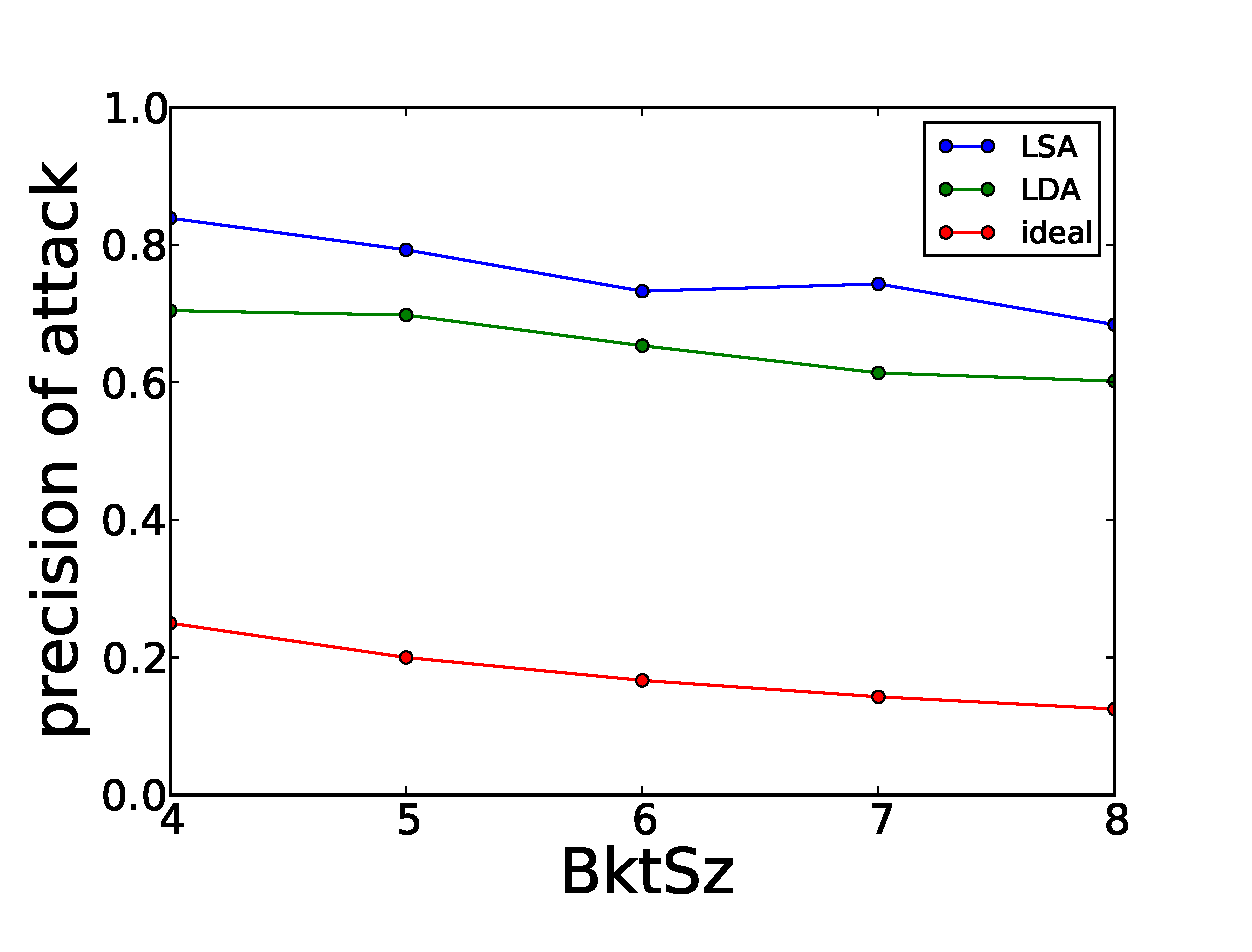
\includegraphics[width=0.9\textwidth]{ETSQ1.eps}
 \vspace{5em}
 \caption{単語バケットに対してメイントピック攻撃の成功率}
 \label{fig:mt1}
 \end{minipage}%
 \begin{minipage}[t]{0.5\linewidth}
 \centering
 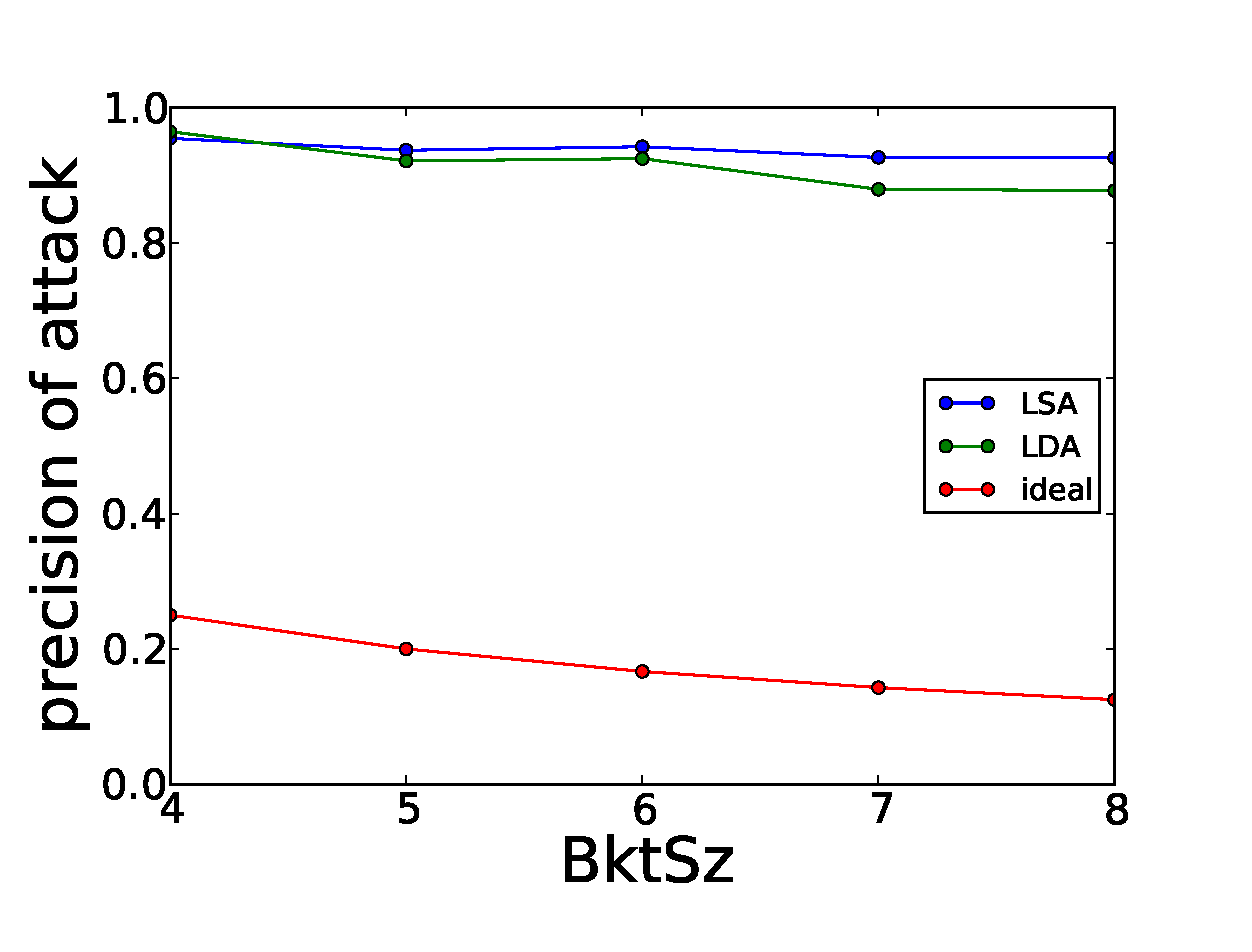
\includegraphics[width=0.9\textwidth]{ETSQ2.eps}
 \vspace{5em}
 \caption{加工した質問のメイントピックと真の質問のメイントピックが一致する確率}
 \label{fig:mt2}
 \end{minipage}
 \end{figure}
 
 単語ごとに$7$個のダミー単語を加えても$60\%$以上の確率で真の質問の単語を見破られる.
 図\ref{fig:mt2}が加工した質問のメイントピックと真の質問のメイントピックが一致する確率を表している.
 ダミー質問の単語を1つトピックに集中しないと真の質問のメイントピックを隠すことが困難であると考えられる.
 
 HDGAはダミートピックの決定し,ダミートピックにおける単語の出現率でランダムに単語を選び真の質問と同じ長さのダミー質問を作る.
 攻撃者が質問者と同様にLDAを用いてメイントピック攻撃する結果が図\ref{fig:mt:HDGA}に示す.
 ここでmaxは質問グループの中で自分のメイントピックの関連値$Pr(\delta_q|q)$が一番高い質問$q$が真の質問である確率で
 minでmaxは質問グループの中で自分のメイントピックの関連値$Pr(\delta_q|q)$が一番低い質問$q$が真の質問である確率である.
 
 \begin{figure}
 \begin{minipage}[t]{0.5\linewidth}
 \centering
 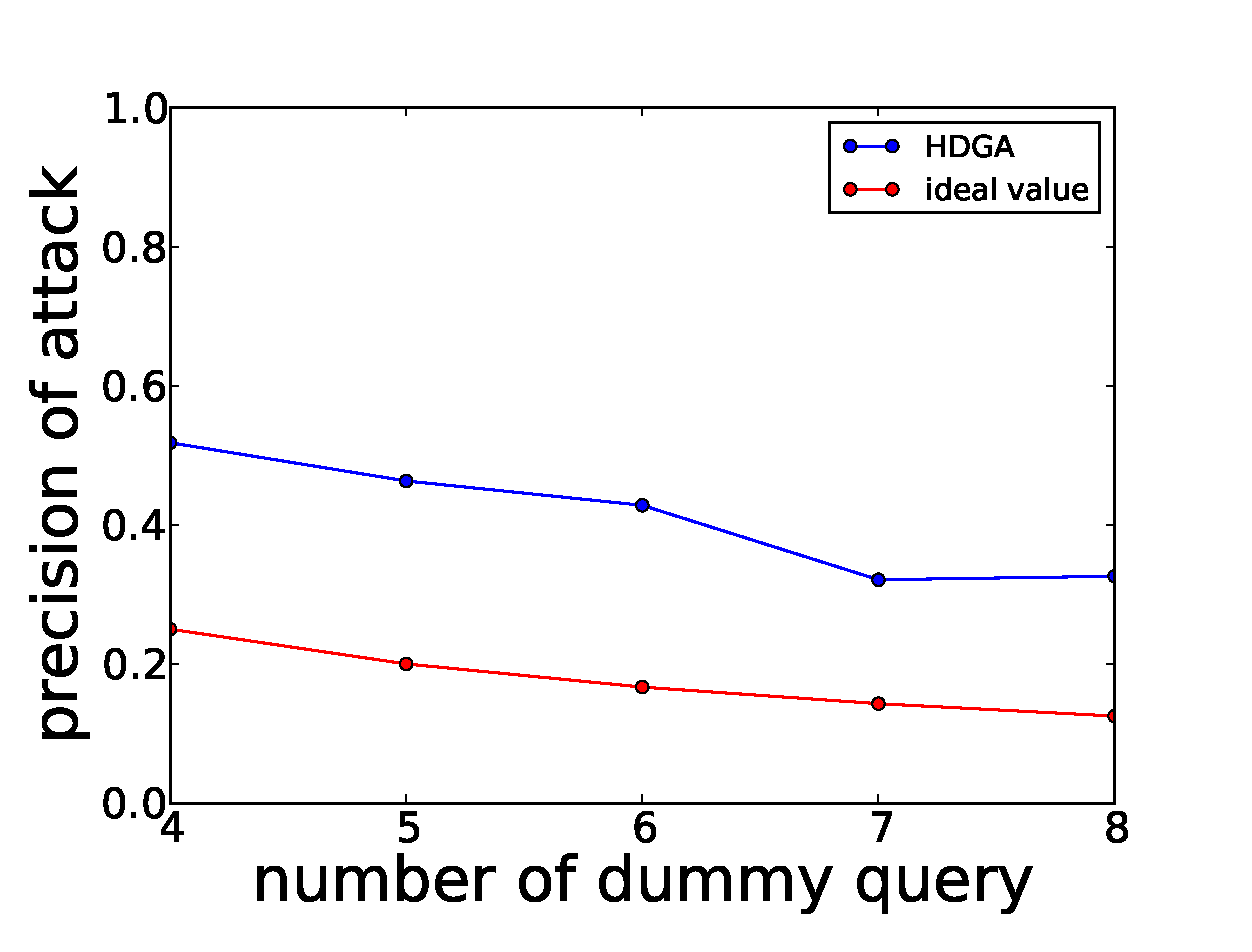
\includegraphics[width=0.9\textwidth]{HMD.eps}
 \vspace{5em}
 \caption{HDGA vs. メイントピック攻撃}
 \label{fig:mt:HDGA}
 \end{minipage}%
 \begin{minipage}[t]{0.5\linewidth}
 \centering
 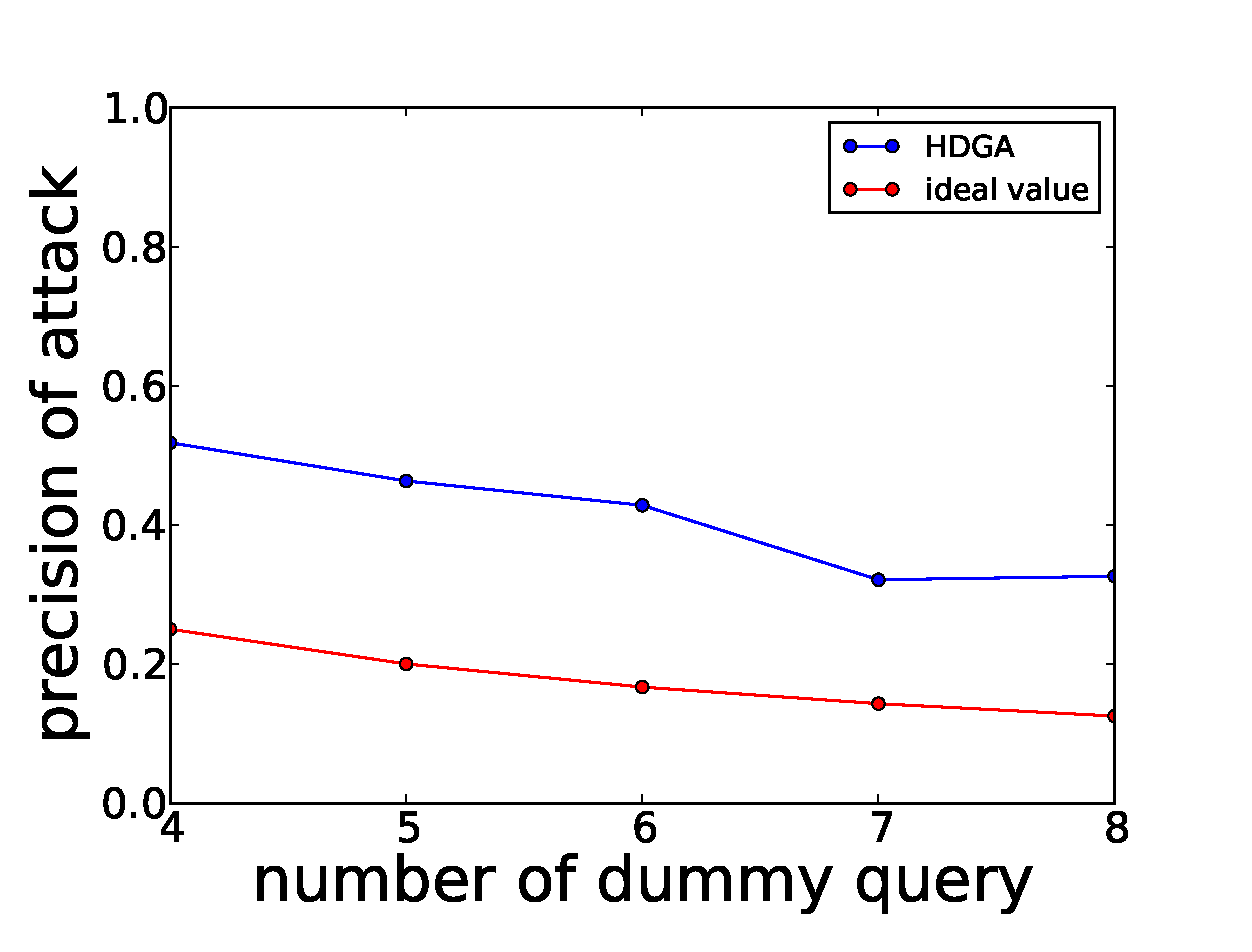
\includegraphics[width=0.9\textwidth]{HMD.eps}
 \vspace{5em}
 \caption{単語バケツ間単語の意味的距離の差,BktSz$=4$}
 \label{fig:r2}
 \end{minipage}
 \end{figure}

 HDGAではダミートピック$t$を決定し,ダミートピックから$Pr(w|t)$に基づにてランダムに単語を選択するため,
 各質問$q$に対してトピック$\delta_q$における確率$Pr(q|\delta_q) = \prod_{w \in q}Pr(w|\delta_q)$の差が少ない.
 しかし,特許検索質問が長いため,
 出現率が高い単語を用いた真の質問$q$が提出される確率$Pr(q) = \prod_{w \in q}Pr(w)$がダミー質問が提出される確率より大きくなり,
 真の質問とその質問のメイントピックの関連値$Pr(\delta_q|q)$が一番低くなると考えられる.

 %また,今までの既存研究では攻撃者が質問者と同じの意味分析手法を用いると仮定するが,
 攻撃者が質問者と同じ意味分析手法を用いて質問曖昧化に対してメイントピック攻撃を行う時,
 1つトピックグループ中のトピック間の距離の影響は\ref{}に示す.
 第\ref{s:sm}章で説明したように,coef距離はトピックの代表単語集合間のDice係数で,
 cos距離はトピックの代表単語集合を意味分析手法を用いて得たトピックベクトル間のcos距離である.

 \begin{table}[!hbp]
 \center
 \begin{tabular}{|c|c|c|c|c|c|}
 \hline
 意味分析手法:ダミトピックの選び方 & rand & cos-near & cos-far & coef-near & coef-far \\
 LDA & 74.9 & 87.5  & 90.1  & 61.0 & 88.9 \\
 LSA &  75.2 & 38.3 & 77.5 & 28.2 & 69.2 \\
 \hline
 \end{tabular}
 \caption{質問曖昧化 vs. MTA}
 \end{table}

 意味的に近いトピックをダミーとピックとすると,
 理想値と近い確率でメイントピック攻撃を防ぐ.
 また,特許文章は曖昧性を生じないように単語を選んでいるため,
 単語の曖昧性をなくす意味分析手法を用いるより,
 直接に単語を用いて距離を計算する方がよりいい結果を得た理由であると考えられる.

 1つトピックグループ中のトピック間の距離
 が
 真の質問とダミー質問の検索結果の一致する割合
 に対する影響は\ref{}に表している.
 真のトピックと意味的に近いトピックをダミートピックにしても質問意図の安全性に影響しないと考えられる.
 
 質問曖昧化のときと同じように攻撃者が質問者と同じ意味分析手法を用いて評価実験した結果はに示す.
 質問曖昧化2は真の質問と同じトピックに属する似たような関連値を持つダミー質問を生成するため,
 メイントピック攻撃では真の質問を見破られない.

 \begin{table}[!hbp]
 \center
 \begin{tabular}{|c|c|c|c|c|c|}
 \hline
 評価方法:ダミー質問数  & 3 & 4 & 5 & 6 & 7    \\
 MTA &  &  &  &  &  \\
 理想 & 25 & 20 & 16.7 & 14.3 & 0.125 \\
 \hline
 \end{tabular}
 \label{tab:mt:HDGA1}
 \caption{質問曖昧化2 vs. MTA}
 \end{table}

 \section{類似攻撃2}

 無効資料タスクで用いた質問は審査感が拒絶した特許文章から抽出されたものであるため,
 特許文章にあるほかの情報も利用できる.
 本論文では1つ会社が出願した特許文章から抽出された質問を
 1人の質問が提出した質問にする.
 類似攻撃2の評価実験は5個以上の質問を提出した質問者について攻撃する.

 ETQSでは1回の検索に対して1つ加工した質問しか提出しないため,
 類似攻撃は対応できない.

 \begin{table}[!hbp]
 \center
 \begin{tabular}{|c|c|c|c|c|c|}
 \hline
 評価方法:ダミー質問数  & 3 & 4 & 5 & 6 & 7    \\
 類似攻撃2 & 98.0 & 97.8 & 97.4 & 97.2 & 96.2 \\
 理想 & 25 & 20 & 16.7 & 14.3 & 0.125 \\
 \hline
 \end{tabular}
 \label{tab:s2:HDGA}
 \caption{HDGA vs. SimAtt2}
 \end{table}

 HDGAは質問グループ間の関連性を配慮していないため,
 図\ref{tab:s2:HDGA}に示すようにダミー質問の個数を7個まで増やしても$96.2\%$で真の質問を見つかる.

 質問曖昧化に対して類似攻撃2を行う時1つトピックグループ中のトピック間の距離の影響は\ref{tab:mt:AAAA}に示す.
 LSAを用いて意味的に近いトピックをダミートピックとすることにより,
 HDGAに比べてよりいい結果を得ることができたが,
 3つのダミー質問に対して$66.8\%$で真の質問を見つかることは安全であると言えない.

 \begin{table}[!hbp]
 \center
 \begin{tabular}{|c|c|c|c|c|c|}
 \hline
 意味分析手法:ダミトピックの選び方 & rand & cos-near & cos-far & coef-near & coef-far \\
 LDA & 94.0 & 95.0  & 93.6  & 95.4 & \\
 LSA &  & 72.7 & 86.0 & 66.8 & 90.3 \\
 \hline
 \end{tabular}
 \caption{質問曖昧化 vs. MTA}
 \label{tab:mt:AAAA}
 \end{table}

 質問曖昧化2では1つ質問グループの中の質問全部1つのトピックに属し,
 質問を持つ単語も意味的近いため,
 類似度攻撃2を防げる.
 その結果は図\ref{}に示す.
 
 \section{類似攻撃}
 類似攻撃の評価実験では類似攻撃2で用いた各質問者の質問からランダムに3つを選び,
 その質問者が攻撃者に知らせれている質問ログとし,
 その質問ログを用いて類似攻撃する.
 
 実験結果は図\ref{}に表している.

 \backmatter% ここから後付
 \chapter{謝辞}%%%%%%%%%%%%%%% 謝辞 %%%%%%%

  %\begin{thebibliography}{}%%%% 参考文献 %%%
  % \bibitem{}
  %\end{thebibliography}
  \bibliographystyle{ieicetr}%           BibTeX を使う場合
  \bibliography{thesis}% BibTeX を使う場合

  \appendix% ここから付録 %%%%% 付録 %%%%%%%
  \chapter{}
  \end{document}
 
 \section{データベース分割}
 
 \begin{table}[!hbp]
 \center
 \begin{tabular}{|c|c|c|c|c|}
 \hline
 評価方法  & SimAtt New & SimAtt LSA  & Maintopic & 重複率  \\
 データベース分割(8)  & 52.3 & 11.6 & 42.1 & 1.5 \\
 \hline
 \end{tabular}
 \caption{データベース分割}
 \end{table} 
 \section{LDA vs LSA}
 
 
  \begin{table}[!hbp]
 \center
 \begin{tabular}{|c|c|c|c|c|c|}
 \hline
 評価方法:ダミー質問数  & 3 & 4 & 5 & 6 & 7    \\
 Maintopic & 98.9 & 98.7 & 98.1 & 98.1 & 97.8 \\
 理想値 & 25 & 20 & 16.7 & 14.3 & 0.125 \\
 \hline
 \end{tabular}
 \label{tab:mt:HDGA2}
 \end{table}

 図\ref{tab:mt:HDGA2}は攻撃者がLSAを用いてメイントピック攻撃する結果を表している.
 LDAモデルのトピックとLSAモデルのトピックは一対一に対応できないため,
 LDAモデルでは1つのトピックに集中している質問がLSAモデルの中でも1つのトピックに集中すると限れない.
 ダミートピックからランダムに生成したデミー質問は真の質問のように複数の意味分析に対応できる強さを持たない.
 
 \begin{table}[!hbp]
 \center
 \begin{tabular}{|c|c|c|c|c|c|}
 \hline
 評価方法:ダミー質問数  & 3 & 4 & 5 & 6 & 7    \\
 SimAtt New &  & 78.2 & 78.5 & 77.3 & 63.8 \\
 SimAtt LSA & 65.5 &55.6 & 50.8 & 48.2 & 50.7 \\
 Maintopic & 75.2 & 72.3 & 67.6 & 64.2 & 58.5 \\
 100番までの検索結果重複率 & 6.0 & 1.9 & 2.0 & 1.9 & 1.9 \\
 \hline
 \end{tabular}
 \caption{SA:LSA ダミートピック選び方:ランダム ダミー質問数の影響1}
 \end{table}

 \begin{table}[!hbp]
 \center
 \begin{tabular}{|c|c|c|c|c|c|}
 \hline
 評価方法:ダミー質問数  & 3 & 4 & 5 & 6 & 7    \\
 SimAtt New &  & 82.8 & 77.0 & 74.4 & 72.6 \\
 SimAtt LSA &  & 52.5 & 47.8 & 43.7 & 42.4 \\
 Maintopic &  & 81.8 & 78.0 & 76.0 & 74.1 \\
 100番までの検索結果重複率 &  & 1.5 & 1.9 & 1.7 & 1.6 \\
 \hline
 \end{tabular}
 \caption{SA:tfidf ダミートピック選び方:ランダム ダミー質問数の影響2}
 \end{table}

 \begin{table}[!hbp]
 \center
 \begin{tabular}{|c|c|c|c|c|}
 \hline
 評価方法:ダミトピックの選び方 & cos-near & cos-far & coef-near & coef-far \\
 SimAtt New & 72.7 & 86.0 & 66.8 & 90.3 \\
 SimAtt LSA & 33.5 & 51.8 & 34.5 & 87.2 \\
 Maintopic &  38.3 & 77.5 & 28.2 & 69.2 \\
 100番までの検索結果重複率 & 2.8 & 2.0 & 2.8 & 1.7 \\
 \hline
 \end{tabular}
 \caption{SA:LSA ダミー質問数:3  ダミトピックの選び方の影響1}
 \end{table}

 \begin{table}[!hbp]
 \center
 \begin{tabular}{|c|c|c|}
 \hline
 評価方法:ダミトピックの選び方 & coef-near & coef-far \\
 SimAtt New & 76.3 & 86.9 \\
 SimAtt LSA & 63.4 & 63.1 \\
 Maintopic  & 77.7 & 87.4 \\
 100番までの検索結果重複率 & 6.5 & 1.3 \\
 \hline
 \end{tabular}
 \caption{SA:tfidf ダミー質問数:3  ダミトピックの選び方の影響2}
 \end{table}


 \chapter{おわりに}

 \backmatter% ここから後付
 \chapter{謝辞}%%%%%%%%%%%%%%% 謝辞 %%%%%%%

  %\begin{thebibliography}{}%%%% 参考文献 %%%
  % \bibitem{}
  %\end{thebibliography}
  \bibliographystyle{ieicetr}%           BibTeX を使う場合
  \bibliography{thesis}% BibTeX を使う場合

  \appendix% ここから付録 %%%%% 付録 %%%%%%%
  \chapter{}
  \end{document}

 \subsection{プライバシー分析}
 PDSでは真の質問$q_u$の代わりに真の質問と一番類似した質問$q_c$を含んでいる質問セットをサーバーに送る。
 $q_c$が真の質問の大半な結果を検索できると考えられ,質問セット中の他の質問をダミー質問に見なす.
 そのため,このメカニズムは検索の精度と再現率に影響を大きく与える.
 また,質問の長さの増加と伴って質問の可能な組み合わせが指数的に増加するため,実践的には特許検索など長い質問が多いテキスト検索と質問拡張に対応できない.


 

 
 
 攻撃者が質問者と違う意味分析手法を用いて攻撃する結果はは\ref{}に表している.
 HDGAに対する評価実験と同じように違う意味分析手法を用い,
 トピックの計算方法を変えることより,
 真の質問がの確率で見破られる.
 
  \begin{table}[!hbp]
 \center
 \begin{tabular}{|c|c|}
 \hline
 符号 & 意味 \\
 \hline
 $W = \{1,2,3, \dots ,N\} $ & 単語集合 \\
 $D = \{1,2,3, \dots ,M\}$ & 文章集合 \\
 $K$ & トピック数 \\
 $T = \{1,2,3, \dots ,K\}$ & トピック集合 \\
 $\ell_i = \{t_1,t_2,\dots,K\} $ & 単語$i$のトピックベクトル \\
 $\ell$ & 質問のトピックベクトル \\
 \hline
 \end{tabular}
 \caption{表記法}
 \end{table}
